\documentclass[12pt,a4paper,titlepage,listof=totoc,bibliography=totoc,chapteratlists=0pt]{scrreprt}

\begin{filecontents*}{\jobname.xmpdata}
	\Keywords{VR, IOT, TODO}
	\Title{Textporfolio}
	\Author{Marcel Pouget}
\end{filecontents*}

\author{Marcel Pouget}
\setcounter{tocdepth}{1}
\usepackage[utf8]{inputenc}
\usepackage[T1]{fontenc}
\usepackage{amsmath}
\usepackage{amsfonts}
\usepackage{amssymb}
\usepackage[table]{xcolor}
\usepackage{graphicx}
\usepackage[left=3.50cm, right=2.00cm, top=2.00cm, bottom=2.00cm,foot=1cm]{geometry}
\usepackage[splitrule,hang,flushmargin,multiple,bottom]{footmisc}
\usepackage{lmodern, textcomp}
\usepackage{lmodern}
\usepackage{pdfpages}
\usepackage[ngerman]{babel}
\usepackage{multicol}
\usepackage{subfig}
\usepackage{float}
\usepackage{array,tabularx,booktabs}
\usepackage{ragged2e}
\usepackage{lipsum}
\usepackage{wrapfig}

\newcolumntype{M}[1]{>{\centering\arraybackslash}m{#1}}

\usepackage{enumitem}
\newlist{compactitem}{itemize}{3}
\setlist[compactitem,1]{label=\textbullet, nosep,leftmargin=1.5em,labelwidth=*,align=left}
\setlist[compactitem,2]{label=--, nosep,leftmargin=1.5em,labelwidth=*,align=left}
\setlist[compactitem,3]{label=\textopenbullet, nosep,leftmargin=1.5em,labelwidth=*,align=left}
\newlist{compactenum}{enumerate}{3}
\setlist[compactenum,1]{label=\arabic*., nosep,leftmargin=1.5em,labelwidth=*,align=left}
\setlist[compactenum,2]{label=\alph*., nosep,leftmargin=1.5em,labelwidth=*,align=left}
\setlist[compactenum,3]{label=\roman*., nosep,leftmargin=1.5em,labelwidth=*,align=left}
\newlist{compactdesc}{description}{3}
\setlist[compactdesc]{leftmargin=1.5em,labelwidth=*,align=left}

\usepackage{microtype}

\usepackage[parfill]{parskip}

\definecolor{bluekeywords}{rgb}{0.13,0.13,1}
\definecolor{greencomments}{rgb}{0,0.5,0}
\definecolor{redstrings}{rgb}{0.9,0,0}
\definecolor{lightgray}{gray}{0.9}
\definecolor{lightblue}{rgb}{0.93,0.95,1.0}

\usepackage{listings}

\makeatletter
\lstdefinestyle{lststyle}{
	basicstyle=%
	\ttfamily
	\lst@ifdisplaystyle\scriptsize\fi
}
\makeatother

\renewcommand{\lstlistlistingname}{List of Listings}
% TODO: define other languages as needed
\lstset{language=Python,
numbers=left,               
numberstyle=\tiny,          
showspaces=false,
showtabs=false,
breaklines=true,
lineskip=-1pt,
tabsize=2,
showstringspaces=false,
breakatwhitespace=true,
escapeinside={(*@}{@*)},
commentstyle=\color{greencomments},
keywordstyle=\color{bluekeywords}\bfseries,
stringstyle=\color{redstrings},
style=lststyle,
xleftmargin=17pt,
         framexleftmargin=17pt,
         framexrightmargin=5pt,
         framexbottommargin=4pt
}
\lstset{
morekeywords={base,var,in,out,dynamic,from,where,select,orderby,function,\$,group,by,into,yield,async,await,@,None,self,as,elif,with}
}
\lstdefinelanguage{TypeScript}{
	keywords={typeof, new, true, false, catch, function, return, null, switch, var, if, in, while, do, else, case, break, void, number, string, boolean, module, \$, export, for, this},
	keywordstyle=\color{blue}\bfseries,
	ndkeywords={class, export, boolean, throw, implements, import, this},
	ndkeywordstyle=\color{darkgray}\bfseries,
	identifierstyle=\color{black},
	sensitive=false,
	comment=[l]{//},
	morecomment=[s]{/*}{*/},
	commentstyle=\color{purple}\ttfamily,
	stringstyle=\color{red}\ttfamily,
	morestring=[b]',
	morestring=[b]"
}
\usepackage{caption}
\DeclareCaptionFont{white}{\color{white}}
\DeclareCaptionFormat{listing}{\colorbox[cmyk]{0.43, 0.35, 0.35,0.01}{\parbox{\textwidth}{\hspace{10pt}#1#2#3}}}
\captionsetup[lstlisting]{format=listing,labelfont=white,textfont=white} 
\captionsetup[table]{justification=centering, singlelinecheck=false}

\usepackage[onehalfspacing]{setspace}

	

\newcommand{\setauthor}[1]{\ohead[]{#1}}

\usepackage[automark]{scrlayer-scrpage}
\pagestyle{scrheadings}
\automark{chapter}
\renewcommand\sectionmark[1]{\markright{\MakeMarkcase {\thesection\hskip .5em\relax#1}}}
\rohead{\ifnum\expandafter\pdfstrcmp\botmark=0 \rightmark\else\leftmark{} --- \rightmark\fi}
\ihead[]{\headmark}
\chead[]{}
\ohead{}
\cfoot[]{}
\ofoot[\pagemark]{\pagemark}
\setheadsepline{.1pt}

\usepackage[hyphens]{url}

\usepackage[a-1b]{pdfx}

\usepackage{hyperref}
\hypersetup{pdfa}

\usepackage[nonumberlist,toc,nopostdot]{glossaries}

\usepackage{chngcntr}
\counterwithout{footnote}{chapter}
\counterwithout{figure}{chapter}
\counterwithout{table}{chapter}
\AtBeginDocument{
	\counterwithout{lstlisting}{chapter}
	\urlstyle{sf}
}
\newcounter{RPages}

\makeatletter
\def\bstctlcite{\@ifnextchar[{\@bstctlcite}{\@bstctlcite[@auxout]}}
\def\@bstctlcite[#1]#2{\@bsphack
	\@for\@citeb:=#2\do{%
		\edef\@citeb{\expandafter\@firstofone\@citeb}%
		\if@filesw\immediate\write\csname #1\endcsname{\string\citation{\@citeb}}\fi}%
	\@esphack}
\makeatother

\clubpenalty=10000
\widowpenalty=10000
\displaywidowpenalty=10000
\interfootnotelinepenalty=10000

\title{Unser tolles Thema -- wir sind suppa}
\author{Stefan Schwammal, Susi Schwammal}

\makeindex
\makeglossaries
\begin{document}
\bstctlcite{IEEEexample:BSTcontrol}
\newcommand{\reminder}[1]
{ \textcolor{red}{<[{\bf\marginpar{\mbox{$<==$}} #1 }]>} }
\newcommand{\icode}[1]{\lstinline$#1$}
%\urlstyle{same}
%\setstretch{1.5}
\setstretch {1.433}
\renewcommand{\arraystretch}{1.2}


\includepdf{./titlepage/coversheet}
\pagenumbering{Roman}
\newpage
\thispagestyle{empty}
\vspace{3cm}
~ \\ \\

Vorwort: 

 

Also, dass hier ist also das berüchtigte Vorwort. ‚Warum?‘ Werdet ihr euch sicher fragen? Warum hat er genau diesen Einstieg gewählt? Ganz einfach. Weil ich mir schwer mit Anfängen tue. Ich muss erstmal was haben, um dann in einen Flow zu kommen, wo die Text dann wie aus einem gebrochenen Damm aus meinen Fingern fließen. Grundsätzlich, wenn es um mein Wissen um die Textsorten geht, fühl ich mich schon ziemlich gut vorbereitet. Wieso? Weil ich gerne schreibe. Egal, ob irgendwelche Kurztexte, bei denen ich die Namen der Personen ändern sollte (tut mir übrigens leid, dass ich Sie eingebaut habe), oder irgendwelche Kommentare, Texte oder anderes. Sogar eine Weiterführung einer Buchreihe wollte ich schreiben, habe schon angefangen, mir die Handlung auszudenken, die Personen zu charakterisieren, und Nebenschauplätze zu entwerfen. Wieso dieses Buch noch nicht in den Regalen von Thalia steht? Weil ich leider bei solchen Projekten nie die Motivation habe, sie fertig zu machen.  

Da ich wirklich viel und gerne lese, habe ich über die Jahre einen guten Eindruck bekommen, wie man eine Geschichte Strukturiert, wie man künstlich Spannung aufbaut, und viele kleine, aber wichtige Details im laufe der Geschichte wieder zur Sprache bringt. Wieso ich dieses Talent nicht nutze? Faulheit. Ich habe meistens nicht die Motivation, mich aufzuraffen und neues zu schaffen. Auch bei der Rechtschreibung habe ich so meine Probleme, vor allem, weil ich mir meine Texte zu selten und ungenau durchlese. Das wird vor allem bei der Diplomarbeit ein Problem werden, dass ist aber noch ein ganz anderes Thema. Ich verlasse mich da einfach viel zu viel auf die technischen Möglichkeiten, und glaube, dass es damit getan ist. Aber im Grunde halte ich mich für einen recht guten Schreiberling, welcher mit etwas Mühe und der richtigen Motivation viel umsetzen könnte. Im laufe der Arbeit wird wahrscheinlich auch genau das mein Problem werden. Weiterzumachen. Mich aufzuraffen. Jeden Tag. Und mich an dieses Dokument zu setzten. Dabei nicht das Leben und meine Liebsten vergessen, sondern mit jedem die Zeit verbringen, die er verdient hat. 

% Hier kommt die Unterschrift drüber
\begin{tabbing}
Leonding, Februar 2022 \hspace{5cm} M. Pouget
\end{tabbing}
\vspace{10cm}
\newpage
\setcounter{page}{1}

%\begin{spacing}{1}
    \chapter*{Abstract}
\end{spacing}
\begin{wrapfigure}{r}{0.3\textwidth}
    \begin{center}
      
\includegraphics[width=0.2\textwidth]{pics/question_mark.png}
    \end{center}
\end{wrapfigure}
Brief summary of our amazing work. In English.
This is the only time we have to include a picture within the text.
The picture should somehow represent your thesis.
This is untypical for scientific work but required by the powers that are.
\lipsum[6]
\newpage
\begin{spacing}{1}
    \chapter*{Zusammenfassung}
\end{spacing}
\begin{wrapfigure}{r}{0.3\textwidth}
    \begin{center}
      
\includegraphics[width=0.2\textwidth]{pics/question_mark.png}
    \end{center}
\end{wrapfigure}
Zusammenfassung unserer genialen Arbeit. Auf Deutsch.
Das ist das einzige Mal, dass eine Grafik in den Textfluss eingebunden wird.
Die gewählte Grafik soll irgendwie eure Arbeit repräsentieren.
Das ist ungewöhnlich für eine wissenschaftliche Arbeit aber eine Anforderung der Obrigkeit.
\emph{Bitte auf keinen Fall mit der Zusammenfassung verwechseln, die den Abschluss der Arbeit bildet!}
\lipsum[6]


\pagestyle{plain}

\renewcommand{\lstlistlistingname}{Quellcodeverzeichnis}

\tableofcontents
\newpage
\setcounter{RPages}{\value{page}}
\setcounter{page}{0}
\pagenumbering{arabic}
\pagestyle{scrheadings}

\begin{spacing}{1}
	\chapter{Erörterung}\label{chapter:introduction}
\end{spacing}
\input{./sections/erörterung.tex}
\begin{spacing}{1}
	\chapter{Kommentar}\label{chapter:introduction}
\end{spacing}
\begin{figure}[h]
    \centering
    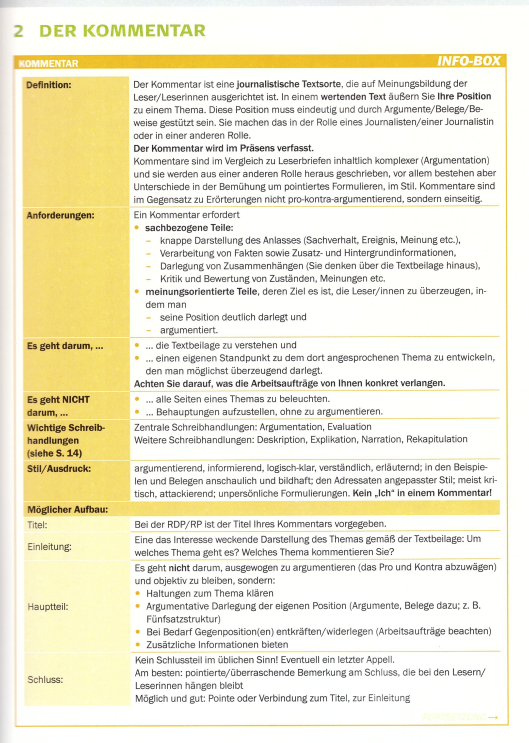
\includegraphics[scale=0.8]{./pics/Screenshot from 2023-02-06 12-27-40.png}
    \caption{Kommentar: Definition + Aufbau}
    \label{fig:impl:Kommentar1}
\end{figure}

\begin{figure}[h]
    \centering
    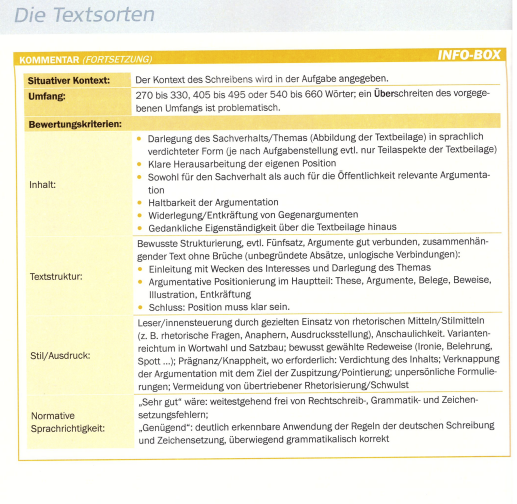
\includegraphics[scale=0.8]{./pics/Screenshot from 2023-02-06 12-27-54.png}
    \caption{Kommentar: Verfassen}
    \label{fig:impl:Kommentar2}
\end{figure}
\begin{figure}[h]
    \centering
    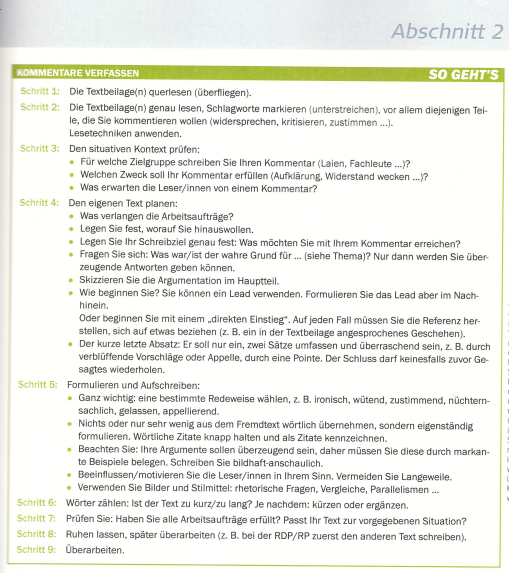
\includegraphics[scale=0.8]{./pics/Screenshot from 2023-02-06 12-28-08.png}
    \caption{Kommentar: Fortsetzung}
    \label{fig:impl:Kommentar3}
\end{figure}


\section{Mustertext}

\subsubsection{Man muss nicht alles haben}

Wahrscheinlich sind nicht alle Leser mit obigem Titel einverstanden. Es gibt zwar viele Einsichtige, die von der Notwendigkeit nachhaltigen Konsums überzeugt sind, aber leider auch viele Andersdenkende, die recht bedenkenlos das Luxusleben der Wegwerfgesellschaft genießen. 

Diese Haltung ärgert Sepp Eisenriegler, der sich als Präsident des Dachverbands für Sozialwirtschaft unermüdlich für soziale und ökologische Aspekte der Nachhaltigkeit und gegen unnötige Vernichtung wertvoller Ressourcen einsetzt. Er versucht die Menschen zu überzeugen, dass die Konsumgier nur dazu treibe, „immer mehr zu arbeiten, um immer mehr Besitztümer anzuhäufen, die man dann gar nicht genießen kann.“ 

 

In diese Falle tappen auch viele junge Menschen, wenn sie über ausreichend Taschengeld verfügen oder mit ihrem ersten selbstverdienten Geld sofort alles kaufen wollen, was als sogenanntes „Must-have“ beworben wird. Man sollte sie von etwas Besserem überzeugen! Aber wie? 

Die Wirkung eines guten Vorbilds gilt als bestes Erziehungsmittel; ein schlechtes bewirkt das Gegenteil. In einer Familie, in der jedes Haushaltsgerät schon beim kleinsten Schaden ohne Reparaturversuch sofort entsorgt und durch ein Neugerät ersetzt wird, wo der Vater alljährlich auf das neueste Automodell umsteigt und die Mutter sich jedem Modediktat beugt, wird auch der Nachwuchs kaum vom aktuellen Dringendwunsch abgebracht und vom Sinn des Sparens überzeugt werden können.  

Doch der Hebel muss auch noch woanders angesetzt werden, nämlich bei der Stärkung eines positiven Selbstbewusstseins. Tatsächlich ist es in der Pubertät oft ziemlich schwer, die eigene Meinung Andersdenkenden gegenüber zu vertreten. Doch mit ein bisschen Mut kann man seinen schon älteren Pullover als „Lieblingskleidung“ verteidigen und es nicht zulassen, dass die persönliche Akzeptanz in der Gruppe vom Besitz aller technischen Neuheiten abhängt. 

 

Erfreulicherweise behaupten viele junge Menschen, theoretisch ein „grünes Herz“ zu besitzen. Doch Worte allein genügen nicht - man muss auch Taten folgen lassen! Bekennt euch deshalb zu der Meinung, dass etwas Gebrauchtes nicht automatisch unbrauchbar ist und dass man nicht alles haben muss, um glücklich zu sein! 

 

313 Wörter 
\section{Eigener Text}

\subsubsection{Werden dicke Menschen dumm? }
In dem Bericht “Fettreiche Ernährung bremst Hirnreifung” geht es um eine Studie, welche die Auswirkungen von fettigem Essen auf Ratten untersucht. Dabei kam ans Licht, das durch zu viel Fett Ablagerung in gewissen Gehirnbereichen entstehen können, welche die Hirnreifung ausbremst. Da der Aufbau von der Ratte dem Menschlichen ähnelt, gab es für die Wissenschaftler Grund zur Sorge. Aus diesem Grund befasse ich mich hier in dem Kommentar, wie man den Konsum von fettreichem Essen vor allem bei Kindern und jungen Erwachsenen bremsen kann. 

 

Als erstes sind die Eltern eines Kindes dafür verantwortlich, was jene in den jungen Jahren zu sich nehmen. Doch viele Eltern möchten ihre Kinder verwöhnen, diese belohnen oder essen selbst gerne ungesundes Essen. Dadurch gewöhnen sich auch die jüngere Generation schnell an das beliebte fast food. Doch wie kann man das verhindern? In meinen Augen sind die Eltern selbst oft nicht gut genug aufgeklärt, was ungesundes Essen alles für negative Auswirkungen auf den menschlichen Körper haben kann. 

 

 Deswegen sollte man schon in den frühen Jahren in der Schule unterrichtet werden, wie man sich und den Körper gesund ernährt, wie man richtig Sport macht und was gesund für einen ist und was nicht. Außerdem würde ich es begrüßen, wenn es für Eltern, die gerade ihr erstes Kind erwarten, Fortbildungen gibt, wie sie ihr Kind richtig ernähren müssen. 

 

Aber natürlich ernähren sich Kinder nicht nur zu Hause bei ihren Eltern. Auch das Essen in der Schule selbst spielt eine wichtige Rolle. Deswegen ist es wichtig, ein anständiges und vor allem gesundes Essen für die Pausen bereitzustellen. In den meisten Schulen gibt es schon Buffets mit reichlich Auswahl, jedoch kommen gesunde und vor allem günstige Menüs immer zu kurz. In den meisten Schulen bekommt man belegte Brötchen oder andere kalte Speisen, aber warme Menüs oder spezielles Essen für Veganer und Vegetarier kommt immer zu kurz. Außerdem sollte das Angebot von ungesunden Essen wie zum Beispiel Pizza oder anderes Fast Food drastisch gesenkt werden. Eine Lösung wäre eine einheitliche Institution, die sich ausschließlich um das Essens-Angebot in Schulen kümmert. Zwar sind schon viele Buffets einer bestimmten Firma, jedoch gibt es da noch immer keine einheitlichen Regeln. 

Mein Appel an die Eltern und vor allem an die Politik: Unterschätzt die Folgen der ungesunden Ernährung bitte nicht. Sorgt für euch und eure Kinder. Und bitte klärt auf, wenn jemand darüber nicht Bescheid weiß! 

Ca 400 Wörter 

\newpage

\section{Formulierungshilfen}
\subsubsection{Einbinden von Informationen }
\begin{compactitem}
    \item "Der/Die Journalist*in XY vertritt in seinem/ihrem Artikel die Meinung, dass..." 
    \item "In dem Artikel XY aus der Tageszeitung XY wird dargestellt..." 
    \item "Das Interview mit dem Forscher XY verdeutlicht..." 
    \item "Eine Umfrage von XY hat ergeben.../...liefert interessante Ergebnisse zum Thema..." 
\end{compactitem}
\subsubsection{Verbinden von Argumenten oder Informationen }
Da Du einen Fließtext verfasst, in dem Du viele Informationen miteinander verknüpfst, sollte diese Verbindung auch sprachlich gekennzeichnet werden. Beispielsweise durch Satzanfänge wie: 
\begin{compactitem}
    \item "Außerdem ..." / "Zudem ..." / "Des Weiteren ..." / "Darüber hinaus ..." / "Folglich ..." / "Demzufolge ..." 
\end{compactitem}
Wenn Du dabei bist, die Gegenargumente zu widerlegen, eignen sich Formulierungen wie: 
\begin{compactitem}
    \item "Allerdings..."/"Jedoch.."/"Aber..."/"Trotzdem..
    \item "Dagegen lässt sich allerdings argumentieren..." 
    \item "Dem gegenüber steht jedoch das Argument..." 
    \item "Trotzdem muss man sagen..." 
    \item "Widerlegen lässt sich diese Behauptung damit, dass..." 
    \item  "Man kann zwar argumentieren, dass... , jedoch/allerdings/aber..."
    \item "Obwohl/Wenngleich behauptet wird, dass... , muss betont werden, dass..."  
\end{compactitem}
\subsubsection{Überleitung zum Fazit }
\begin{compactitem}
    \item "Zusammenfassend kann man sagen..." 
    \item "Es wird deutlich..." 
    \item "Die Studien/Untersuchungen/Befragungen zeigen/ergeben eindeutig..." 
    \item "Anhand dieser Punkte zeigt sich also..." 
    \item "Es steht außer Frage, dass..." 
    \item "Wie sich erkennen lässt..." 
\end{compactitem}
\subsection{Realitätsbezug: }
Der Kommentar findet sich vor allem in der Zeitung wieder. Hier findet man oft Kommentare (oder Leserbriefe) zu aktuellen Themen. Weitere Beispiele wären in sozialen Medien, Onlineforen, Kundenbewertungen und viele mehr. 


\subsection{Erklärung}

Ein Kommentar ist ein textliches Stellungnahme zu einem bestimmten Thema, Ereignis oder Text. Ein Kommentar drückt die Meinung des Autors über das besprochene Thema aus und versucht, es zu bewerten oder zu interpretieren.

Er ist in der Regel kürzer als eine Erörterung oder eine Argumentation und kann sowohl subjektiv als auch objektiv sein. Ein objektiver Kommentar bezieht sich auf Fakten und Informationen und versucht, eine sachliche Bewertung zu geben, während ein subjektiver Kommentar die persönliche Meinung des Autors zum Ausdruck bringt.



\subsection{Beispiele für verwandte Textsorten}
Glosse, Leitartikel, Rezension, Kolumne, Leserbrief, Erörterung
\subsection{Abgrenzung} Ausgesprochen elaborierte Leserbriefe können einem Kommentar
ähnlich sein, weisen jedoch seltener die inhaltliche Komplexität
(Argumentation) eines Kommentars auf. Ähnlichkeiten zur Erörterung
im argumentativen Vorgehen stehen Unterschiede in der Präsentation der Argumente, in der Art der eigenen Positionierung und im Stil
gegenüber.
\subsection{Umfang}
270 bis 330, 405 bis 495 oder 540 bis 660 Wörter

\subsection{situativer Kontext}erforderlich
\subsection{Eigene Erfahrung}Auch diese Textsorte fällt mir nicht so schwer. Auch hier ist es hautpsächlich wichtig, faktisch richtig zu Argumentieren, und freundlich zu bleiben.


\begin{spacing}{1}
	\chapter{Leserbrief}\label{chapter:introduction}
\end{spacing}
\begin{figure}[h]
    \centering
    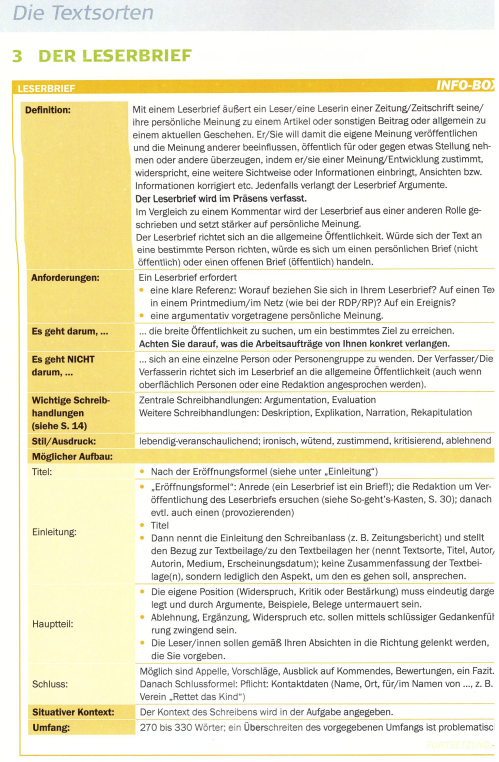
\includegraphics[scale=0.8]{./pics/Screenshot from 2023-02-06 12-28-25.png}
    \caption{Leserbrief: Definition + Aufbau}
    \label{fig:impl:Leserbrief1}
\end{figure}

\begin{figure}[h]
    \centering
    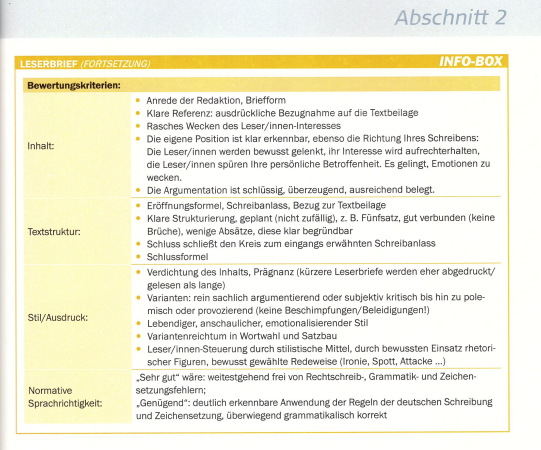
\includegraphics[scale=0.8]{./pics/Screenshot from 2023-02-06 12-28-55.png}
    \caption{Leserbrief: Verfassen}
    \label{fig:impl:Leserbrief2}
\end{figure}
\begin{figure}[h]
    \centering
    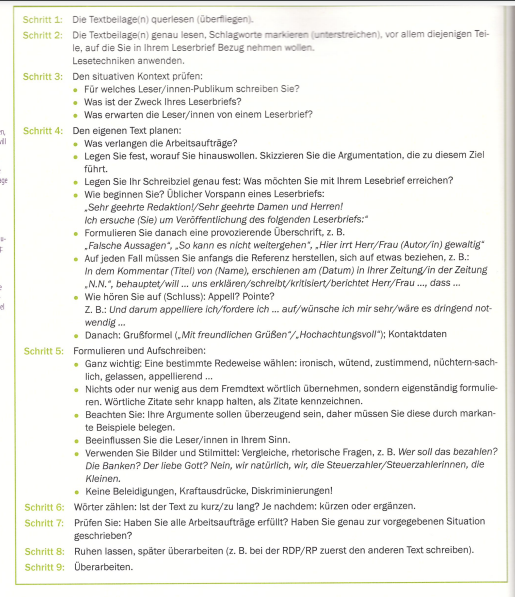
\includegraphics[scale=0.8]{./pics/Screenshot from 2023-02-06 12-29-05.png}
    \caption{Leserbrief: Fortsetzung}
    \label{fig:impl:Leserbrief3}
\end{figure}



\section{Mustertext}

Sehr geehrte Redaktion! 

Ich ersuche Sie um die Veröffentlichung des folgenden Leserbriefs: 
\subsubsection{Sexy und sexistisch  Muss das sein? }

Als ich die Kolumne „Sexy und sexistisch“ von Niki Glattauer, erschienen am 18. März 2013 in der Tageszeitung Kurier las, schoss mir sofort eine Frage durch den Kopf: Muss sowas denn wirklich sein?  

Herr Glattauer berichtet von einem sexistischen Werbeplakat der Wiener Linien. Darauf ist ein Mann zusehen, der seinen Allerwertesten direkt auf zwei elegant gekleidete Frauen, welche sich gerade unterhalten, gerichtet hat. Dabei sagt die eine Frau kichernd zu der anderen: Ich sagte doch, du sollst mehr Bus fahren. Niki Glattauer dreht daraufhin die Situation um und erläutert, dass ein Plakat mit zwei Männern in Anzug, die über den Hintern einer Frau feixen, ohne Berechtigung, als sexistisch oder unpassend abgestempelt werden würde. Herr Glattauers betont, dass ein klarer Unterschied zwischen sexy und sexistisch besteht. Denn das einzige, das vom Werbeplakat betont wird, ist der Hintern des Mannes. Kein Mann muss sich dadurch belästigt fühlen.  

Man kann das Ganze jedoch auch anders sehen. Die Ansicht, die man mit der Thematik verbindet, ist immer abhängig von den Gedanken oder Erinnerungen der Person. Manche Menschen ärgern sich über die Werbung und meinen sie sei unpassend und wieder andere lachen darüber und denken sich nichts weiter dabei.  

Da Sexismus leider auch heute noch immer eine sehr große Rolle in unserer Gemeinschaft spielt, muss man doch nicht mehr Wirbel über das Thema verbreiten, als ohnehin schon besteht. Ich gebe Herrn Glattauer mit der Überlegung, dass sexy nicht gleich sexistisch meint, zwar recht, jedoch kann man doch auf diese Anspielungen bei einer Werbung verzichten. Viele Leute fühlen sich dadurch persönlich angegriffen, beschämt oder gar verletzt und wohin sollen diese Gefühle bei der Debatte des Sexismus führen?  

\section{Eigener Text}
\subsection{Angabe}
\subsubsection{Körperbilder }

Verfassen Sie einen Kommentar. 

Situation: Im Rahmen eines Projekts Ihrer Klasse bzw. Ihres Kurses zum Thema Körperbilder verfassen Sie einen Kommentar, der auf der Projektwebsite veröffentlicht wird und für den Sie auch einen passenden Titel formulieren. 

Lesen Sie den Bericht Beauty-Apps: Die Macht der Influencer von Selina Thaler aus der OnlineAusgabe der Tageszeitung Der Standard vom 26. Jänner 2019 (Textbeilage 1). Verfassen Sie nun den Kommentar und bearbeiten Sie dabei die folgenden Arbeitsaufträge: 

\begin{compactitem}
    \item Geben Sie wieder, wodurch Selbstwahrnehmung und Körperbild laut Textbeilage beeinflusst werden.  
    \item Nehmen Sie dazu Stellung. 
    \item Bewerten Sie im Text genannte Maßnahmen und Initiativen, um der dargestellten Problematik entgegenzuwirken. 
\end{compactitem}

Schreiben Sie zwischen 270 und 330 Wörter. Markieren Sie Absätze mittels Leerzeilen.

\subsubsection{Beauty-Apps: Die Macht der Influencer }

Der Artikel von Selina Thaler über die Auswirkungen von Sozial Media und vor allem bearbeitet Bilder auf junge Frauen war einer der informativste Artikel, den ich seit Langem gelesen habe. Und dennoch frage mich, wieso ist das angesprochene Problem in der heutigen, aufgeklärten Zeit immer noch so ein Problem? 

Konkret geht es um die Auswirkungen, welche retuschierte Bilder auf unser Gehirn haben. Welche Folgen dies haben kann und dass es sogar Depressionen und starke Eifersucht auslösen kann. Und das ganz unterbewusst, ohne dass die Nutzer etwas davon mitbekommen. Vor allem die Vorbildfunktion der Influencer spielt hier eine starke Rolle. Viele jugendliche Mädchen, die selbst oft noch kein Selbstwertgefühl haben, wollen oft so perfekt aussehen wie die Menschen auf den Selfies auf Instagram. Snapchat-Dismorphia nennt man diese Unzufriedenheit, die durch die Verbreitung falscher und bearbeiteter Bilder ausgelöst wurden. 

Trotz geplanter Gegenmaßnahmen finde ich es schrecklich, dass durch Apps wie Instagram ein solch falsches Bild von dem menschlichen Körper an junge Menschen geliefert wird. Es ist schlimm, dass sich Mädchen abhungern oder Essstörungen aufbauen, nur um genauso dünn zu sein wie Models im Internet oder im Fernsehen. Doch viele dieser Fotos sind einfach bearbeitet und entsprechen nicht der Realität. Ich finde es gut, dass es schon Versuche gibt, solche Bilder zu markieren oder Models mit „Schönheitsfehler“ zu nehmen. Trotzdem müsste man meiner Meinung schon im Kindesalter die Menschen aufklären und über solche Fallen informieren. Denn trotz jeder Markierung, das Gehirn vergleicht sich trotzdem unterbewusst immer mit anderen. 

Ich rufe Sie, liebe Leser, dazu auf, ihre Söhne und Töchter darüber aufzuklären! Jeder sollte wissen, wie falsch Menschen auf Sozial Media sind, wie viele falsche Sachen viel zu viel Aufmerksamkeit bekommen, und vor allem, dass jeder Körper schön ist. Egal wie er geformt ist, wie viel man wiegt und wie groß die Kurven von jemanden sind. 

302 Wörter 

\newpage


\section{Formulierungshilfen}

Aufbau eines Leserbriefs: 
\begin{compactitem}
    
    \item Anrede: z.B. Name des Redakteurs: Sehr geehrter Herr Schuster! 
    \item Genaue Angabe des Artikels, auf den du dich beziehst: Datum und Überschrift des Artikels, Erscheinungsort 
    \item Schreibabsicht 
\end{compactitem}
So könntest du beginnen: 
\begin{compactitem}
    \item Sie schreiben in Ihrem Artikel (Titel) vom (Datum), der (wo) erschienen ist, dass ….. Dazu möchte ich Ihnen Folgendes mitteilen: … 
    \item Mit Interesse habe ich Ihren Artikel (Titel) vom (Datum) im (Ort) gelesen und frage mich … 
    \item Ihr Beitrag zum Thema … berührt mich sehr. Auch ich habe ähnliche Erfahrungen gemacht. 
    \item In Ihrem Artikel (Titel) vom (Datum) schreiben Sie, dass … 
    \item In seinem Beitrag schreibt Herr Huber, dass … 
    \item Endlich war in Ihrer Zeitung zu lesen, was ich mir schon immer gedacht habe: … 
    \item Ihr Artikel (…) erscheint mir inhaltlich wichtig, schon alleine deshalb, weil 
\end{compactitem}
Im Hauptteil beurteilst du 
\begin{compactitem}
    \item Auch ich habe den Eindruck, dass 
    \item Auch ich habe diese Erfahrung gemacht … 
    \item  Diese Situation kenne ich sehr gut … 
    \item Diese Aussagen entsprechen auch meinen Erfahrungen 
    \item Diese Meinung / Sichtweise kann ich ganz und gar nicht teilen.  
    \item Ich sehe das überhaupt nicht so wie Herr Huber! 
\end{compactitem}
\subsection{Realitätsbezug}
Leserbriefe (Textsorte) findet man oft in Zeitungen oder Zeitschriften, besonders in Print-Medien. Sie dienen als Plattform für die Meinungen und Ansichten der Leser zu aktuellen Themen oder Ereignissen. Leserbriefe können auch in Form von Online-Kommentaren auf Nachrichtenwebsites oder in sozialen Medien veröffentlicht werden. 

\subsubsection{Beispiele für verwandte Textsorten}
offener Brief, Posting
\subsubsection{Abgrenzung}
Der offene Brief richtet sich nicht an ein konkretes Medium (z.B. um
diesem zu widersprechen), sondern an eine breite Öffentlichkeit; dabei
bedient er sich mitunter eines Mediums, ohne auf dessen Berichterstattung Bezug zu nehmen.
\subsubsection{Umfang} 270– 330 Wörter
\subsubsection{situativer Kontext} erforderlich

\begin{spacing}{1}
	\chapter{Meinungsrede}\label{chapter:introduction}
\end{spacing}
\begin{figure}[h][p]
    \centering
    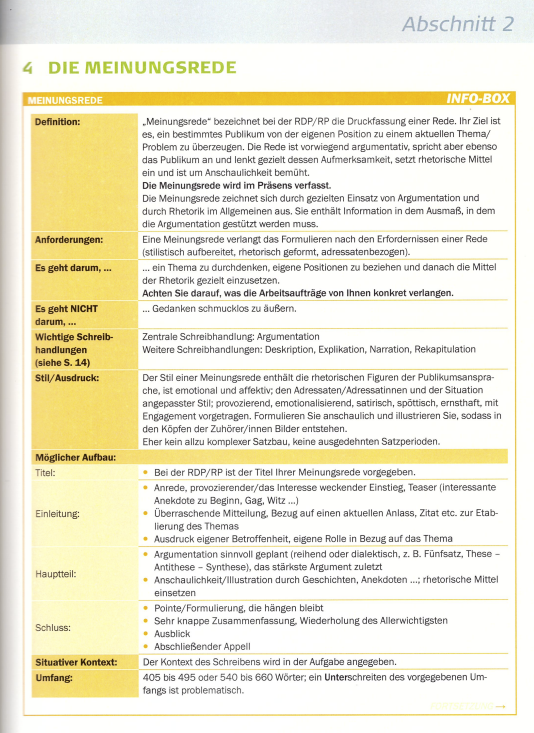
\includegraphics[scale=0.8]{pics/Screenshot from 2023-02-06 12-29-34.png}
    \caption{Meinungsrede: Definition + Aufbau}
    \label{fig:impl:Meinungsrede1}
\end{figure}

\begin{figure}[h][p]
    \centering
    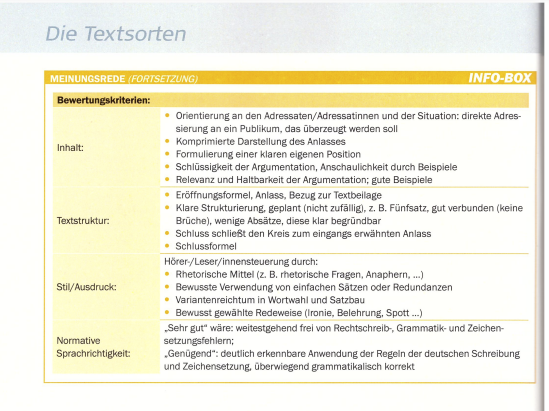
\includegraphics[scale=0.8]{pics/Screenshot from 2023-02-06 12-30-22.png}
    \caption{Meinungsrede: Verfassen}
    \label{fig:impl:Meinungsrede2}
\end{figure}
\begin{figure}[h][p]
    \centering
    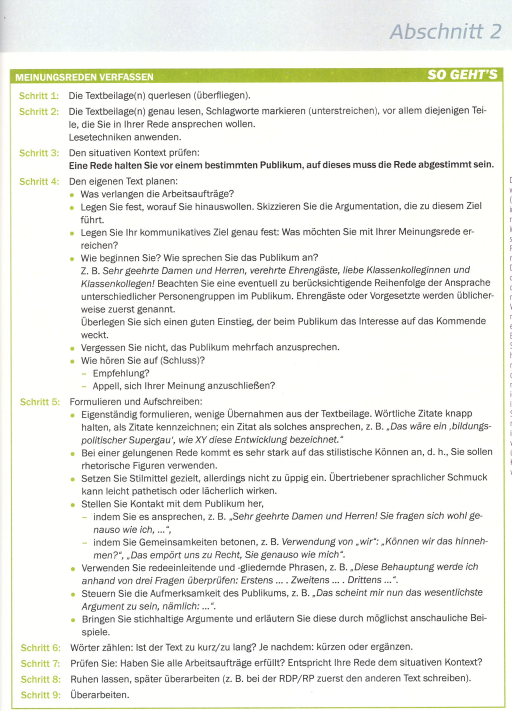
\includegraphics[scale=0.8]{pics/Screenshot from 2023-02-06 12-30-34.png}
    \caption{Meinungsrede: Fortsetzung}
    \label{fig:impl:Meinungsrede3}
\end{figure}

\section{Mustertext}
\subsubsection{Meinungsrede Zivilcourage}
Du blödes Kameradenschwein! Diese Aussage ist an niemanden im Publikum gerichtet, sondern fällt häufig im Umfeld von Menschen, die Zivilcourage beweisen. Doch, was ist das eigentlich, Zivilcourage? Viele kennen diesen Begriff nur aus Appellen von Politikern und Kirchenvertretern. Doch obwohl sie so wichtig ist und von so vielen gepredigt wird, ist sie fast nicht mehr in unserer Gesellschaft aufzufinden.  

Ich möchte zuallererst einen Fall aus den 60ern in den USA, genauer gesagt in Queens, neu aufrollen. Das Opfer ist Catherine „Kitty“ Genovese, eine Junge Frau, die eines Nachts mitten auf den Straßen New Yorks erstochen wird. Tja, spöttisch könnte man nun sagen, in den USA kann alles möglich werden. Der Täter war Winston Moseley. Dieses unmenschliche Monster hat nicht nur die Frau auf offener Straße, umringt von aufwachenden Anwohnern mit einem Jagdmesser erstochen, nein. Er kam später zurück, und stach erneut zu. Um seine Grausamkeiten noch abzurunden, vergewaltigte er die leblosen Überreste der armen Frau. Bitte bedenken Sie, dass dies immer noch mitten auf offener Straße geschah! In der Zwischenzeit hat niemand der dort Wohnenden seinen Allerwertesten hochbekommen, oder die Polizei verständigt. Und da soll man sich noch auf die Straße trauen? Muss man immer davon ausgehen, dass man von niemandem Hilfe bekommen wird? Leidet die Gesellschaft unter dem „bystander effect“? 

Dieser besagt nämlich, dass wir zu Herdentieren geworden sind. „Also, wenn die andern nichts machen, dann mach ich auch nichts“ – oder ähnliche Aussagen kommen dabei heraus. Die Menschen fürchten sich davor, sich zu blamieren und gehen davon aus, irgendjemand wird schon aufstehen und handeln. Verwunderlich, da wir doch alle die Superhelden aus Film und Fernsehen verehren und gerne wären wie sie. Die zeigen nämlich noch wirklich, was Zivilcourage ist, und dazu müssen sie nicht mal die Welt retten. Es reicht schon, wenn sie eine unschuldige Zivilistin retten. Der bystander effect ist der Bösewicht in unserem Blockbuster, und er ist nicht alleine. An seiner Seite kämpfen auch noch das Verlangen nach Harmonie, sowie der Drang nach Komfort. Sieht nicht gut aus für unseren Superhelden. Ob das ein Happy End wird? 

Fakt ist doch, wir wollen alle komfortabel leben. Und ein Außenseiter will man schon in der Volksschule nicht sein. Also immer schön mit dem Strom schwimmen, ja nicht anders sein und auffallen. Tarnkappenmodus aktiveren und unter dem Radar fliegen. Kurz gesagt: keiner will aus der Masse herausstechen. Es gilt als merkwürdig, und für manche auch als abstoßend, wenn jemand anders als der Rest ist. Doch genau hier sehe ich den Fehler. Es ist das „Mindset“, die Einstellung, die uns allen eingeprägt wird. Genau diese Barriere haben wir alle in unserem Gehirn. Nur die, die sie überwinden, können den anderen ein Vorbild sein. Doch um dieses annehmen zu können, müssen wir alle uns dazu bewegen, dieses Hindernis zu überwinden, zumindest es zu versuchen. Wir können nicht die Gesellschaft verändern, doch das muss auch nicht sein. Wir können und müssen uns selbst verändern, nur so kann die Meinung der Herde langsam gedreht werden.  

Um diesem Vortrag einen guten Ausklang zu verleihen, möchte ich Sie alle etwas bitten: Schauen sie nicht weg.  
Auch wenn es unangenehm ist: Schauen Sie nicht weg.  
Auch wenn es „schon jemand anders machen wird“: Schauen Sie nicht weg.  

Handeln Sie. 

535 Wörter 

\section{Eigener Text}
(Text aus dem Unterricht)
\subsubsection{Warum Sozialmedia nicht immer nur unterhaltsam und lustig ist. }

Wissen Sie, wer alles ihren Kindern heimlich über Social-Media Textnachrichten sendet? Theoretisch könnte es jeder sein. Ihr Nachbar, Ihre Schwester, selbst ihre Katze könnte anonym verstörende Nachrichten an die Kleinen versenden. Denkt denn keiner an die Kinder? Wie viele Bedrohungen und Beleidigungen die Kleinen wohl schon ertragen mussten? Wissen Sie, welchen Effekt unzensiertes Nutzen des Internets auf sich hat? Sehr geehrte Eltern, wann haben Sie das letzte Mal wirklich über die Gefühle Ihrer Kinder gesprochen? Heute geht es darum, wie Sie sich und vor allem ihre Kinder von äußerem Einfluss über die sozialen Medien schützen können. Denkt doch einmal an die Kinder. 

 

Es ist wie mit dem Masturbieren. Jeder tut es, keiner redet darüber. Wer von euch – und jetzt bitte ehrlich sein, – wer von euch war noch nie auf einem sozialen Netzwerk? Hat sich noch nie ein Video auf Youtube angesehen oder einen Post auf Facebook geliket? Jeder von uns, ja, wirklich jeder weiß, wovon ich spreche. Soziale Medien verändern unseren Alltag, verändern unsere Denkweise. Aber denkt wirklich keiner hier an die Kinder? An diejenigen, die ihre ganze Entwicklung noch vor sich haben, an die, bei denen der Einfluss von außen am meisten fruchtet? Keiner redet davon, wie sehr große Influencer auf TikTok oder Instagram die Jugend manipuliert. Für ihre Zwecke einsetzt. Welche Zwecke werden Sie sich jetzt fragen.  

Ganz einfach. Geld verdienen. Die Placements so gestalten, dass sie vor allem die junge Generation in die Irre führt und sie zum Kauf sinnlos teurem March bewegt. Auch die Denkweise, die freie Meinung und vieles andere kann von so bekannten Leuten schnell verändert werden. Und egal ob bewusst oder unbewusst, Menschen mit einer großen Reichweite haben eine sehr große Macht. Damals im Nationalsozialismus war es am Anfang nicht viel anders. Jeder schwimmt mit dem Strom, und der Rest hat Angst, darin unterzugehen, wenn er sich in die andere Richtung bewegt. Denkt doch einmal an die Kinder! 

Corona, die Ukraine, Russland oder die USA. Jeder bekommt immer die neusten Bilder, sieht grausame Videos aus Kriegsgebieten oder macht sich selbst zu einem Virologen. Soziale Medien haben unsere Art zu denken und Informationen auszutauschen, komplett verändert. Jedoch bekommen schon die Kleinsten von uns alles mit, – da sehr viele Wissenskanäle und Nachrichtenchannels auch online ihre Nachrichten ausstrahlen. Und da – wie jeder weiß, vor allem schlechte Nachrichten sich wie warmes Brot verkaufen, kann man auch hier wieder nur sagen: Denkt denn wirklich keiner mehr an die Kinder? An unsere Zukunft? 

Glauben Sie denn, es ist vorteilhaft, wenn die Kleinen von Anbeginn ihres Lebens mit schlechten Nachrichten konfrontiert werden? Wenn sie immer nur negative Sachen hören, gewalttätige Videos sehen oder in den Fokus von irgendwelchen Spaßvögeln geraten, welche sich daran aufgeilen, Menschen mit Drohungen Angst zu machen? Außerdem ist es als Elternteil sehr schwer zu kontrollieren, ob nicht irgendwelche pädophilen Menschen mit den Kleinen schreiben. Die sind dann meist noch so jung, dass sie nicht mal wissen, in welcher Gefahr sie sich befinden. Denkt doch einmal an die Kinder und schützt sie vor dem Einfluss von sozialen Medien 

 

Der letzte Punkt ist ganz kurz zusammengefasst: Mobbing. Über soziale Medien ist es schon fast Pflicht geworden, einen zweiten Account zu erstellen, mit dem man nicht in Verbindung gebracht werden kann. Und mit dieser Anonymität ist es dann ein Leichtes, einem Freund “Du H*rensohn” in die Kommentare zu schreiben. Der User wird sich nur denken, hach, das war lustig, während sein Freund vielleicht schwer von der Beleidigung getroffen ist. Auch hier denkt keiner an die Kinder. An diejenigen, bei denen Mobbing besonders groß und verbreitet ist. An diejenigen, welche durch Beleidigungen den größten Schaden anrichten. Auch hier kann ich nur an die Eltern appellieren: schränken sie den Gebrauch von sozialen Medien ein. Den Ihrer Kinder, aber auch Ihren eigenen. Soziale Medien können so viel Leid verursachen, und das alles nur, weil ein paar gute Programmierer mit der größten Schwäche des Menschen gespielt haben. Sie wollen Anerkennung. (Und vielleicht ein bisschen Geld muhahaha) 

\newpage

\section{Formulierungshilfen}
\subsubsection{Die Einleitung}
\begin{compactitem}
    \item … soll lebendig formuliert sein, da sie der erste Eindruck Ihres Textes ist und zum Weiterlesen / Zuhören animieren soll. Ein Trick der Rhetorik ist es, dass man Aufmerksamkeit durch Lachen oder Verstörung (= Provokation) erweckt. 
    \item  … soll das Thema beinhalten und erklären, warum Sie zu diesem Problem eine Rede halten. 
    \item    … ist von der Themenstellung abhängig. 
    \item  ... eindeutig den Redeanlass wiedergibt - hier sollte schon klar sein, welche Meinung Sie vertreten.  
\end{compactitem}
\subsubsection{Der Hauptteil}
\begin{compactitem}
    \item … ist der längste und ausführlichste Teil Ihrer Rede. 
    \item … enthält nur Argumente, die Ihre Meinung untermauern. Ein Trick der Rhetorik ist es, dass Gegenargumente angesprochen werden, aber als nichtig abgetan werden, um der eventuellen Gegenkandidatin / dem eventuellen Gegenkandidaten den Wind aus den Segeln zu nehmen. [Beispiel: Hier könnten wir natürlich auch … ins Treffen führen, aber das führt zu nichts, weswegen ich hier nicht näher darauf eingehen möchte.] 
    \item … soll auf das Auditorium Bezug nehmen und in diesem Teil wird es auch immer wieder gezielt angesprochen. Achtung! Sie müssen die Situierung genau lesen, denn wenn Sie als Schüler/in/ Ihre Schulkolleg/innen ansprechen, dann werden Sie diese sicherlich nicht Siezen. Andererseits würden Sie die Direktorin / den Direktor oder Vorgesetze wahrscheinlich nicht duzen. 
    \item … soll rhetorische Mittel enthalten, um die Argumentation zu unter-stützen. [Anm.: Sie sollten sich hier nicht unnötig in Panik versetzen, da wir generell in Figuren sprechen. Es gibt 160 000 verschiedene Stilmittel, aber Sie werden höchstwahrscheinlich mit den gängigsten punkten können. 
\end{compactitem}
\subsubsection{Im Schlussteil}
\begin{compactitem}
    \item  … soll das Wesentliche kurz zusammengefasst werden. 
    \item    … soll ein Appell oder gar ein Lösungsvorschlag an das Publikum ge-richtet werden. Das entnehmen Sie aber den Arbeitsaufträgen! Beachten Sie hier, dass Sie unbedingt das Verbum "appellieren" verwenden! Beachten Sie die Zielgruppe - an wen wendet sich meine Rede?
\end{compactitem}

\subsection{Realitätsbezug}
Die Rede kommt vor allem in der Politik vor, und ist ein sehr wichtiger Bestandteil, um eine große Anzahl der Menschen für sich zu entscheiden.  

\subsection{Erklrärung}

Eine Meinungsrede ist eine Textsorte, bei der eine Person ihre Meinung zu einem bestimmten Thema oder einem aktuellen Ereignis öffentlich äußert. Meinungsreden werden oft vor einem Publikum gehalten, wie beispielsweise bei politischen Veranstaltungen, Kundgebungen oder öffentlichen Diskussionen.

Sie sollte gut vorbereitet und überzeugend sein, um das Publikum zu überzeugen und seine Meinung zu beeinflussen. Eine Meinungsrede muss klar und verständlich formuliert sein, damit das Publikum sie versteht, und sollte auch emotionale und logische Argumente enthalten, um das Publikum zu überzeugen.



\subsection{Beispiele für verwandte Textsorten}Gelegenheitsrede, Überzeugungsrede, Feierrede, Ansprache, politische Rede, Aufruf
\subsection{Abgrenzung} Die Meinungsrede zeichnet sich durch ihren gezielten Einsatz von
Argumentation und Rhetorik im Allgemeinen aus. Sie ist dabei nicht
zwingend politisch oder an einem politischen Anlass orientiert, wie
etwa die politische Rede. Die eigene Position steht bei der Meinungsrede im Vordergrund, sie wird jedoch untermauert und das Publikum
miteinbezogen. Sie informiert und erklärt nur so weit, wie notwendig,
um die Argumentation zu stützen.
\subsection{Umfang} 405 bis 495 oder 540 bis 660 Wörter
\subsection{situativer Kontext} erforderlich
\subsection{Eigene Erfahrung} Die Schwierigkeit hängt ganz von der Aufgabenstellung ab. Wenn es ein Thema ist, zu dem ich eine feste und klare Meinung habe, ist es kein Problem, mit Argumenten mein Gegenüber zu überzeugen. Bei unbekannten Themen tu ich mir jedoch schwerer, da ich dann kaum Argumente finden kann.

\begin{spacing}{1}
	\chapter{Textanalyse}\label{chapter:introduction}
\end{spacing}
\begin{figure}[h][p]
    \centering
    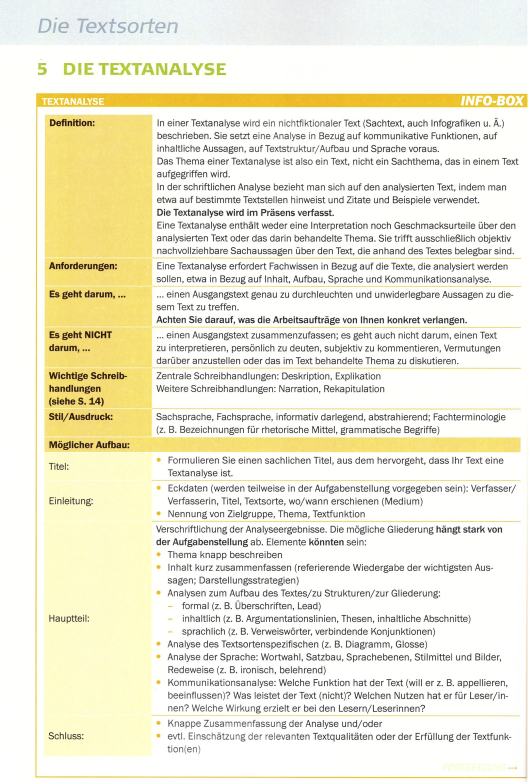
\includegraphics[scale=0.8]{pics/Screenshot from 2023-02-06 12-30-44.png}
    \caption{Textanalyse: Definition + Aufbau}
    \label{fig:impl:Textanalyse1}
\end{figure}

\begin{figure}[h][p]
    \centering
    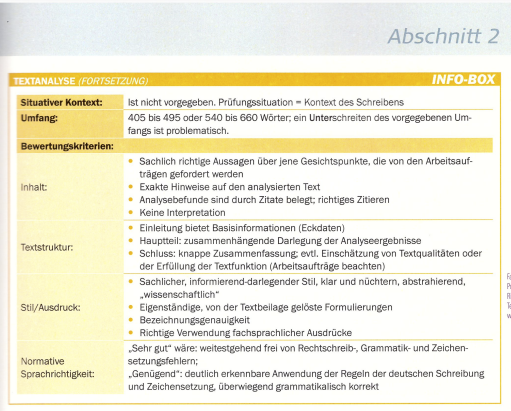
\includegraphics[scale=0.8]{pics/Screenshot from 2023-02-06 12-30-55.png}
    \caption{Textanalyse: Verfassen}
    \label{fig:impl:Textanalyse2}
\end{figure}
\begin{figure}[h][p]
    \centering
    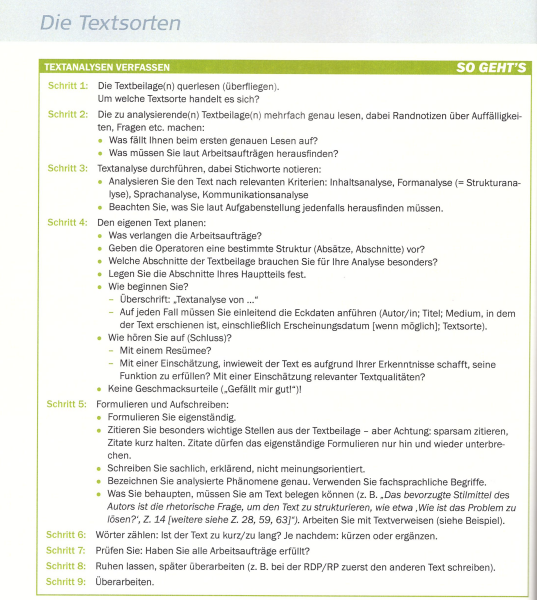
\includegraphics[scale=0.8]{pics/Screenshot from 2023-02-06 12-31-09.png}
    \caption{Textanalyse: Fortsetzung}
    \label{fig:impl:Textanalyse3}
\end{figure}

\section{Mustertext}
\subsubsection{Textanalyse: „Der Unsinn von der „Work-Life-Balance“}
Die Verbesserung der Work-Life-Balance ist ein Vorschlag, der bereits seit einiger Zeit als Lösungsansatz für Menschen verwendet wird, die in der Arbeit unzufrieden sind. Der Autor Robert Betz erklärt in seinem Artikel vom 20.12.2013 auf der Website „Focus online“, warum er dieses Prinzip unsinnig findet und es „letztendlich jedoch zu noch mehr Stress und Erschöpfung der Betroffenen“ (Z. 10 f.) führe. Er spricht damit die ArbeitnehmerInnen des Landes an und versucht mit seinem Text zum Umdenken zu bewegen.  

Robert Betz beginnt die Kolumne mit dem Aufstellen seiner These, dass die Work-Life-Balance Unsinn sei. Danach bringt er in mehreren Absätzen mit Überschriften unterschiedliche Argumente für seine These vor. Zum Beispiel behauptet er, dass man durch die „Abwertung der Arbeit und der Zeit, die wir in ihr verbringen“ (Z. 18 f.) das Opferbewusstsein verstärkt. Auch erläutert er, dass unser Körper auf unsere Einstellungen und Gedanken reagiert und man mit unterdrückten Gefühlen Unordnung im Arbeitsumfeld stiften kann. Sein letztes Plausibilitätsargument ist, dass „der Mensch kein Monaden- oder Einzelwesen, sondern ein Gemeinschaftswesen“ (Z. 57 ff.) sei und es einem „innere Befriedigung und damit Zufriedenheit“ (Z. 56 f.) gibt, wenn man mit anderen gemeinsam etwas erreicht.  

Wie sich an den bereits erwähnten Zitaten erkennen lässt, finden sich kaum sprachliche Auffälligkeiten. Die von Robert Betz verwendete Sprachebene ist die Schriftsprache, wobei er manchmal an der Grenze zur Umgangssprache steht (z. B. „Das gibt ihm eine […]“, Z. 56 f.; „Hier der inkompetente Chef, […]“, Z. 65 f.). Vordergründig wirkt der Text neutral und sachlich, jedoch lassen sich bei genauerem Hinsehen auch subjektive Wertungen und sprachliche Ausreißer erkennen. Dies zeigt sich vor allem in den Ich-Formulierungen („Ich behaupte, der Mensch […], Z. 52 f.; „Hierbei ist nicht entscheidend, welche Arbeit ich verrichte […]“, Z. 70 ff.). Allerdings spricht der Autor seine Leserschaft gekonnt an und bringt viele Beispiele, die jedem aus dem Alltag bekannt vorkommen (vgl. Z. 32 ff). Um die Alltagstauglichkeit des Textes noch weiter zu steigern, verwendet Robert Betz kaum Fachbegriffe. Eine Ausnahme stellt hier das Wort „Monaden“ (Z. 58) dar, welches er in der Fußzeile erläutert. Die Kolumne wurde auch mit einigen rhetorischen Figuren ergänzt. Zum Beispiel lassen sich eine Klimax (z. B. Z. 18 – 30, Z. 52 – 56, Z. 66 – 74) oder eine Emphasis (z. B. „An unserem Arbeitsplatz verbringen […]“, Z. 32 ff.; „Wer mit einer negativen Einstellung […]“, Z. 81 ff.) finden. Diese tragen zur Verdeutlichung der Relevanz bei und schaffen es bei der Leserschaft Aufmerksamkeit zu erregen. Die Emphasen werden durch den asyndetischen Satzbau noch deutlicher unterstrichen, was sich am Beispiel „[…] Gefühle wie Angst, Wut, Enttäuschung, Neid, Eifersucht […]“ (Z.83f) erkennen lässt.  

Um die Intention des Autors klarer zu machen, soll nun noch ein Blick auf den Aufbau des Textes gerichtet werden. Der Artikel besitzt keine klassische Einteilung, da der Schlussteil einer typischen Kolumne (zusammengefasste Meinung des Autors/der Autorin) fehlt. Dieser ist aber auch nicht notwendig, da der ganze Text informierend und aufklärend, wie ein Bericht, wirken soll. Es gibt einen stetig steigenden Spannungsbogen und der Höhepunkt befindet sich am Schluss, da hier ein Blick in die Zukunft jedes Arbeiters/jeder Arbeiterin geworfen wird. Dies hängt mit der Argumentationsstrategie des Autors zusammen, bei welcher er von seinen schwächsten zu den stärksten Argumenten übergeht. Diese Aneinanderreihung wirkt ebenso, wie die gewählte Sprache, spannend auf den Leser/die Leserin.  

Laut Robert Betz wird die Arbeitszeit von der einzelnen Person als unfreie Zeit wahrgenommen. Man arbeitet nur, um Geld zu verdienen und „niemand würde freiwillig arbeiten, wenn er nur genug Geld hätte, außer vielleicht ein paar freischaffenden Künstlern“ (Z. 21 ff.). Hier kommt die aufklärende Natur des Artikels ins Spiel. Die Leserinnen und Leser des Textes werden gut über die Schattenseiten der Work-Life-Balance als Lebensmotto informiert. Doch trotz der guten Aufklärung und einiger passender Beispiele, fehlen konkrete Lösungsansätze. Nichtsdestotrotz ist dieser Text ein guter Einstieg, um ArbeiterInnen davon zu überzeugen, dass die Work-Life-Balance Unsinn sei.  

650 Wörter 
\section{Eigener Text}
\subsubsection{Text 1}
\subsubsection{Textanalyse: „Der Unsinn von der „Work-Life-Balance“}
In dem Leserbrief „Der Unsinn von der „Work-Life-Balance“ von Robert Betz geht es um die Thematik Work-Life-Balance. Der Artikel ist am 20.12.2013 bei dem Publisher „Focus“ erschienen. Der Autor ist ein Diplom-Psychologe, Coach und Therapeut, welcher sich gut in seinen Fachgebieten auskennt.  

Wie teilen Sie sich ihre Freizeit auf? Sorgen Sie dafür, dass ihre Arbeitszeiten ausgewogen sind? Und das Wichtigste: Wie fühlen Sie sich dabei? Denn um genau das geht es in dem Artikel. Kurz zusammengefasst kritisiert der Autor den Unsinn der Work-Life-Balance, vor allem, weil durch die Einstellung viele Menschen ihre Arbeitszeit nicht mehr als Lebenszeit sehen und sich dadurch das Arbeitsklima in der Firma verschlechtert. Man hat weniger Lust zu arbeiten und leistet weniger.  

Der Text ist in 5 Kapitel unterteil, welche (bis auf die Einleitung) alle Argumente gegen den Ausdruck „Work-Life-Balance“ scharf kritisieren. Die Argumente sind gut belegt und strukturiert aufgebaut. Da der Artikel von Anfang an seinen Standpunkt festlegt, gibt es keinen Spannungsbogen oder Pro und Kontra Argumente. Der Text beginnt mit einer kleinen Einleitung und einer Studie, welche belegt, dass sich die physische Befindlichkeit der Menschen stetig verschlechtert. Danach folgen 4 Argumente gegen den neuen Trend der Work-Life-Balance.    Im letzten Absatz geht es noch darum, wie der Autor die Zukunft sieht und wie man das Schlimmste verhindert. 

Die Sprache ist sehr sachlich gehalten, es gibt kaum Fremdwörter und keine unklaren Begriffe. Die vom Autor gewählte Sprache ist die Schriftsprache, welche alles sehr gut verständlich macht, der Leserbrief richtet sich dadurch an ein sehr großes Publikum und ist zeitlos geschrieben. Da es keine besonderen Stilmittel gibt, liest sich der Text wie ein Sachtext.  

Der Autor möchte mit dem Leserbrief die jetzige Generation von Arbeitern warnen und für die zukünftigen Arbeitnehmer Schlimmeres verhindern, da sich nachweislich die Gesundheit der Menschen immer mehr verschlechtert. Deswegen richtet sich der Appel am Ende an eine große Masse, hauptsächlich natürlich an die arbeitenden Menschen. 

Zusammenfassend kann man sagen, dass der Psychologe den Artikel sehr übersichtlich und sachlich aufgebaut hat und klare, gut strukturierte Argumente gegen die Work-Life-Balance gebracht hat. Gleichzeitig hat er alle offenen Fragen beantwortet und seine Aussagen mit den Quellen belegt. 
\subsubsection{Text 2:}
\subsubsection{Häme macht uns zu schlechteren Menschen }
Was ist eigentlich Häme und was macht sie so gefährlich? Um genau diese und auch noch weiter Fragen geht es in dem Text “Häme macht uns zu schlechteren Menschen” von Mercedes Lauenstein, welcher in dem Online-Magazin “Jetzt” erschienen ist. “Häme, sagt Wikipedia, ist eine Kombination aus Schadenfreude, Besserwisserei und Sadismus” (11-12, Tetbeilage1). Und um genau geht es: Wie viele Menschen mit Schadenfreude überkleine Fehler Anderer versuchen, ihr eigenes Leben schön zu reden, zu verbessern und ihre eigenen Sorgen auszublenden. Doch ist es wirklich immer einfacher über andere zu lästern als eine neue Form der Freundlichkeit zu etablieren? Der Text ist in einzelne Abschnitte unterteilt, wobei jeder Abschnitt ein Thema abgeschlossen behandelt. Die Einleitung acht deutlich, um was es in dem Artikel geht, und sie versucht Spannung aufzubauen. Da der zweite Absatz eine Erklärung zu dem Wort Häme ist, beginnen erst im dritten Abschnitt die Argumente gegen die Einstellung zu der Lebensweise. Die Argumente sind dabei unterhaltsam aufgebaut, enthalten aber auch interessante Informationen, welche leider nicht belegt sind. Auch einen Strukturierten Aufbau der Argumente, welcher sich durch den Text zieht, sucht man hier vergeblich. 

Die Autorin benutzt eine recht eigene Sprache, die sehr von zusammengesetzten Wärtern durchzogen ist. Phrasen wie “eine dermaßen Läster-Hysterie” (54, Textbeilage 1) und “Manufactum-Kunden” (9, Textbeilage 1) sind keine Seltenheit. Auch Aussagen wie “zu Tode verspottete Klischees” (19, Textbeilage 1) sind Beispiele dafür, wie die Autorin mit Hyperbeln arbeitet, um dem Leser den Nonsens der Häme klarzumachen. Auch “Kokosfreundin” (35, Textbeilage 1) sind Phrasen, welche nicht im alltäglichen Sprachgebrauch zu finden sind. Hier handelt es sich um die Vermenschlichung und eine Hyperbel, welche passend in den Text eingearbeitet wurden. 

Der Artikel ist mit einer sehr jungen Ausdrucksweise (siehe 35, Textbeilage 1) geschrieben worden, welche schon fast zu der Jugendsprache zählt. Die Sprache ist sehr unterhaltsam, auch wenn sich der Text durch die vielen zusammengesetzten Wortgruppen nicht sehr flüssig lesen lässt. Durch die sehr besondere Schreibweise ist die Zielgruppe des Textest die jüngere Generation, auch wenn der Inhalt jeden Leser betrifft. 

Doch was möchte der Autor mit seinen Aussagen jetzt eigentlich aussagen? Naja, sein größtes Zeil ist es, die neuen Verhaltensmuster zu durchbrechen, den Menschen wieder einen Touch von Freundlichkeit einzureden, und sie darauf aufmerksam zu machen, dass Häme schneller abhängig machen kann als man glaubt. Viele Menschen sollten einfach ihre Ausdrucksweise überdenken, da man dieselben Tatsachen auch nett, freundlich und sachlich ausdrücken kann. Man muss sich nicht immer an dem Leid der anderen ergötzen, wenn man auch mit ein bisschen Freundlichkeit dasselbe und noch so viel mehr erreichen kann. 

Zusammenfassend kann man sagen, dass dem Autor ein wirklich unterhaltsamer und informativer Text gelungen ist, welcher jedoch erst am Ende seine wahren Absichten zeigt und nicht sehr einfach zu lesen ist. Der Autor verwendet eine Sprache, die einen Großteil der Jüngeren Menschen anspricht. Jedoch sollte der Test auch für die ältere Generation interessant gemacht werden, und dafür bräuchte man eine andere Ausdrucksweise.

\newpage

\section{Formulierungshilfen}
Einleitung

\begin{compactitem}
    \item Der Roman/die Kurzgeschichte (Testsorte) „ABC“ (Titel) von XY (Autor) wurde 19 veröffentlicht (Erscheinungsjahr). 
    \item Der Roman/die Kurzgeschichte/der Text behandelt das Thema X... (Thema) 
    \item Der Text beleuchtet das Thema X kritisch, indem er... (Deutungsansatz) 
    \item Der Text kann verstanden werden als... (Deutungsansatz) 
    \item In der folgenden Analyse möchte ich untersuchen, inwiefern... (Deutungsansatz)
\end{compactitem}
Hauptteil
\begin{compactitem}
    \item Das Kapitel XY thematisiert eine zentrale Fragestellung des Romans, indem... 
    \item An dieser Stelle im Text wird deutlich, dass ... 
    \item In Zeile „Nummer“ beginnt ... 
    \item Der Text beginnt mit ... 
    \item  Im Verlauf des Romans wird deutlich, dass... 
    \item Im Gegensatz zum Anfang des Romans... 
    \item  Die Textstelle „Zitat“ ist kennzeichnend für die Figur X, da hier deutlich wird, dass... 
    \item In Zeile XY wird indirekt deutlich, dass die Figur... 
    \item Es besteht ein Konflikt zwischen ... 
    \item An dieser Stelle wird deutlich, dass ... 
    \item Spannung wird aufgebaut durch ... 
    \item An dieser Stelle wird die Frage aufgeworfen, ob ... 
    \item „Zitat“ unterstreicht, dass ... 
\end{compactitem}
Schluss / Fazit
\begin{compactitem}
    \item Zusammenfassend lässt sich sagen, dass ... 
    \item  Mein eingangs formulierter Deutungsansatz hat sich insofern (nicht) bestätigt, als dass... 
    \item Es bleibt offen/der Autor lässt offen, ob ... 
    \item Der Leser fragt sich, ob ... 
    \item Insgesamt gibt der Text einen Überblick über ... 
    \item Insgesamt lässt sich über den Text/das Gedicht sagen, dass ... 
    \item Der Text hinterlässt beim Leser den Gedanken/das Gefühl, dass … 
    \item  Das Ende des Textes ist offen, weil … 
\end{compactitem}


\subsection{Realitätsbezug}
Kommt immer dann vor, wenn ein Text analysiert wird. Wenn z.B. jemand einen bestimmten Text oder eine Geschichte bewerten möchte, wird die Person sich die Eigenschaften des Textes ansehen und analysieren. Außerdem ist es eine beliebte Form, um literarische Texte und Gedichte zu analysieren.
\subsection{Erklärung}

Eine Textanalyse einer Meinungsrede bezieht sich auf die systematische Untersuchung einer Meinungsrede, um ihren Inhalt, ihre Struktur und ihre Wirkung auf das Publikum zu bestimmen. Dabei kann man eine Meinungsrede aus verschiedenen Perspektiven analysieren, wie zum Beispiel aus sprachlicher, argumentativer oder emotionaler Sicht.


\subsection{Beispiel für verwandte Textsorten} Textinterpretation
\subsection{Abgrenzung} Anders als die Textinterpretation, die ihrerseits auf einer Analyse aufbauen muss, ist die Analyse nicht interpretativ. Sie bleibt auf der Ebene
des analytisch Feststellbaren und befasst sich umso genauer mit den
Aspekten der Analyse. Die Zusammenfassung bzw. eine etwaige
Bewertung im Schlussteil muss auf den belegten Analyseergebnissen
basieren und objektiv, bzw. intersubjektiv, nachvollziehbar sein;
persönliche Geschmacksurteile sind der Textanalyse fremd. 

\subsection{Umfang}405 bis 495 oder 540 bis 660 Wörter

\subsection{situativer Kontext} Kein von der Prüfungssituation abweichender Kontext 
\subsection{Eigene Erfahrung} Auch eine der schwereren Textsorten, da man wirklich genau auf den Text eingehen muss, und die ganzen Stilmittel, rhetorischen Figuren und anderen wichtige Abschnitte erkennen muss. Wenn man sich davor ansieht, was dabei wichtig ist, ist diese Textsorte aber kein Promlem.

\begin{spacing}{1}
	\chapter{Textinterpretation}\label{chapter:introduction}
\end{spacing}
\begin{figure}[h]
    \centering
    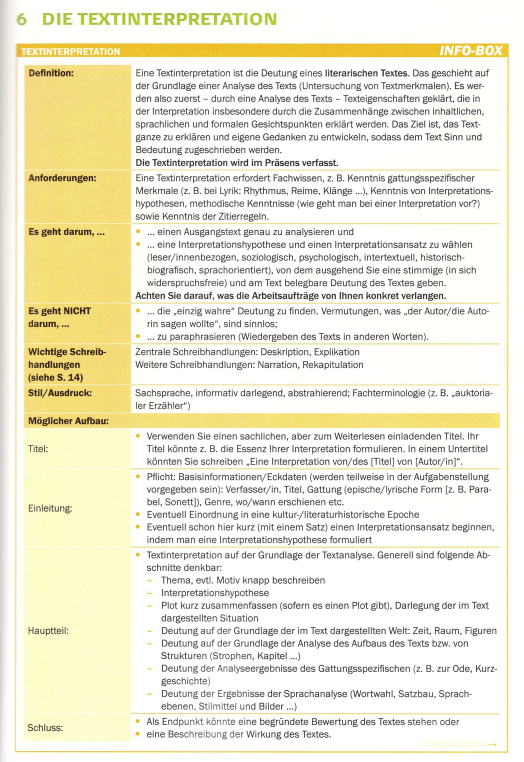
\includegraphics[scale=0.8]{./pics/Screenshot from 2023-02-06 12-31-18.png}
    \caption{Textinterpretation: Definition + Aufbau}
    \label{fig:impl:Textinterpretation1}
\end{figure}

\begin{figure}[h]
    \centering
    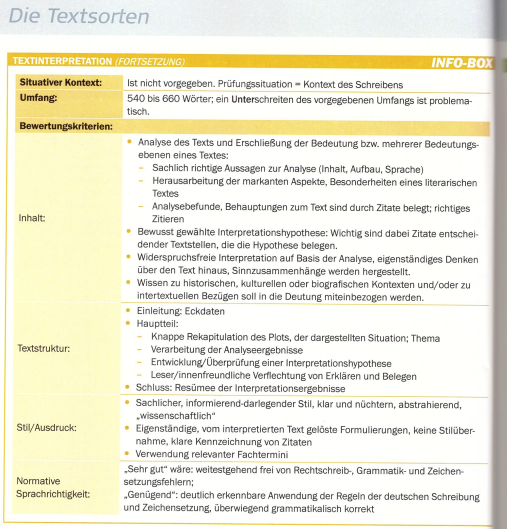
\includegraphics[scale=0.8]{./pics/Screenshot from 2023-02-06 12-31-28.png}
    \caption{Textinterpretation: Verfassen}
    \label{fig:impl:Textinterpretation2}
\end{figure}
\begin{figure}[h]
    \centering
    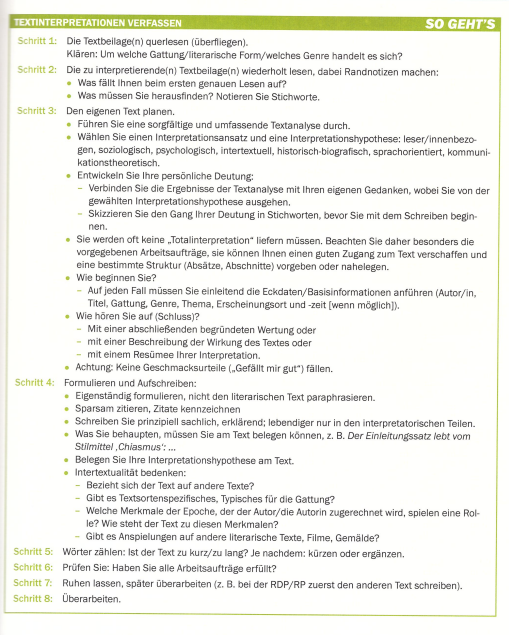
\includegraphics[scale=0.8]{./pics/Screenshot from 2023-02-06 12-32-23.png}
    \caption{Textinterpretation: Fortsetzung}
    \label{fig:impl:Textinterpretation3}
\end{figure}



\section{Mustertext}

\subsubsection{Nichts ist unpräziser als Gerechtigkeit }
Eine Interpretation von „Lieferung frei Haus“ von Günter Kunert 

In der Kurzgeschichte „Lieferung frei Haus“, die 1988 in „Arbeitstexte für den Deutschunterricht. Deutsche Kurzgeschichten 11. – 13. Schuljahr“ erschien, beschreibt Günter Kunert die Tücken einer Welt, in der absolute Gerechtigkeit herrscht, und stellt gleichzeitig die Frage, ob man einen Menschen für alle Folgen seines Handelns verantwortlich machen kann.  

Anfangs wird beschrieben, wie anonyme Lastwägen in der Dämmerung Holzkisten an verschiedenste Haushalte ausliefern. Dies geschieht auch im Haus, in dem Friedrich W. Schmall, der Hauptcharakter, wohnhaft ist. Im Vorbeigehen bemerkt er den Empfänger, der diese Lieferung voller Entsetzen entgegennimmt. Schmall wird schon bald von der Portiersfrau aufgeklärt, beim Inhalt der Kisten handle es sich um Leichen. Dieses absurde Vorkommnis wird ihm von der Bäckersfrau bestätigt, deren Mann ebenfalls eine Leiche in Empfang nehmen musste. Es handelt sich um eine Greisin, die dieser auf regennasser Straße mit seinem Auto tötete. Schmall kann sich einen Anflug von Freude über diese ausgleichende Gerechtigkeit nicht verkneifen. Auf der Straße trifft er auf eine Menschenmenge, die beobachtet, wie ein Ex-Soldat, der Deserteure erschoss, vierzig Kisten geliefert bekommt. Danach bekommt Schmall erstmals Zweifel an den Akteuren und der moralischen Rechtfertigung hinter diesen Lieferungen. Als er seine Verlobte besuchen will, bekommt auch sie eine solche Lieferung. Er flüchtet, ohne mit ihr zu sprechen. Als er sie später darauf anspricht, rechtfertigt sie sich, doch er flüchtet wieder. Die Geschichte endet damit, dass auch Friedrich W. Schmall eine Holzkiste geliefert bekommt, die seine Verlobte beinhaltet. Sie konnte den Verlust ihres Mannes nicht verkraften und nahm sich das Leben.  

Die Kurzgeschichte ist aus der Perspektive eines personalen Erzählers geschrieben, der die Handlung linear wiedergibt und stets im Präteritum bleibt. Sprachlich fallen besonders die Beschreibungen der Personen auf, besonders die Beschreibungen der Empfänger der Holzkisten im Moment der Übergabe sind sehr lebhaft und vermitteln ein fast schon überzeichnetes Bild des Entsetzens. So vergleicht er etwa das Gesicht eines Empfängers mit einer „bleichen, großen Blase“, die mit „zwei schwarzen Knöpfen“ besetzt sei (Z 28 – 30). Der groteske Effekt der Lieferung einer Leiche an einen normalen Haushalt wird so nochmals verstärkt, da auch die Empfänger als leichenähnlich beschrieben werden.  Sprachliche Besonderheiten sind auch in der letzten Szene vorhanden, in der Friedrich W. Schmall selbst zum Empfänger wird.  Der Autor verlängert die Zeit künstlich, und die Erzählzeit wird um ein Vielfaches länger als die erzählte Zeit. Auch werden die handelnden Personen als teilnahmslos dargestellt, so etwa Friedrich W. Schmall, der „ohne das Gefährt zu beachten“ (Z188) sein Haus betritt, oder auch die Lieferanten, „aus deren Unbeweglichkeit ihn die Augen reglos anglotzten“ (Z196). Dieser leblose Ablauf wird durch die lebhafte Überzeugung der Hauptfigur, dass es sich bei der Lieferung um einen Irrtum handeln müsse, unterbrochen. Als er allerdings seine Verlobte in der Kiste erkennt, resigniert er nach „einer von den kleineren Ewigkeiten“ (Z214), was nochmals eine Zeitdehnung darstellt.  

In der Kurzgeschichte wird eine absolute moralische Kraft in eine anderweitig normale Welt eingeführt. Diese absolute moralische Kraft besteht aus den Lieferanten der Kisten beziehungsweise ihren Auftraggebern, die entscheiden, wer Schuld am Tod der Verstorbenen hat. Diese Entscheidungen werden von amtlicher Seite getroffen (Z.64), und von niemanden in Frage gestellt. Besonders nicht von den Empfängern der Kisten, da diese oftmals zu schockiert über die Schuldzuweisung sind, und diese möglichst vor der Öffentlichkeit verbergen möchten. Auch für beobachtende Passanten ist es leichter, die Empfänger als Schuldige darzustellen, als mit ihnen zu sympathisieren, da so die Annäherung an eventuelle Mörder argumentativ verteidigt werden müsste. Dieser Mechanismus schützt die Kräfte hinter den Auslieferungen und ihre Entscheidungen vor jeglichen öffentlichen Verurteilungen. Dadurch ähnelt das beschriebene System autoritären Regimen, in denen Regierungen oder Behörden Entscheidungen treffen können, die einzelne Bürger stark negativ betreffen, ohne selbst Konsequenzen fürchten zu müssen. Friedrich W. Schmall zeigt hierzu im Verlauf der Geschichte drei typische Einstellungen der Bevölkerung zu diesen Umständen. Anfangs ist er noch erfreut darüber, dass dem Bäcker Gerechtigkeit widerfährt (Z72). Später stellt er allerdings die Möglichkeit fest, dass auch Irrtümer geschehen könnten und dass solche Schuldentscheidungen nie wirklich gerecht gefällt werden können. Schließlich erfährt er am eigenen Leib, wie es ist, die Schuld am Tod eines Mitmenschen zugesprochen zu bekommen. Bemerkenswert ist hierbei auch, dass die exekutierenden Personen ihre Aufgabe ohne Gewissensbisse erledigen, und die Liste der angeblichen Mörder als normal abzuarbeitende Aufgabe betrachten (Z. 219). Dieses Abweisen von Schuld ist wiederum ein typisches Kennzeichen von autoritären Strukturen. 

Diese Diskussion der Schuld in all ihren Facetten, insbesondere in autoritären Strukturen, wie sie im Laufe der Geschichte immer wieder auftrat, gelingt dem Autor in dieser Kurzgeschichte äußerst prägnant. Er stellt Fragen, die auch in unserer heutigen Gesellschaft noch nicht gelöst sind, und die jeder Leser für sich selbst beantworten muss. 

\section{Eigener Text}
\subsubsection{Als die Turmuhr halb drei schlug}

“Die Küchenuhr”, eines der bedeutendsten Werke der Trümmerliteratur, ist ein Auszug aus der Prosasammlung “An diesem Dienstag”. Diese wurde von dem Autor Wolfang Borchert 1947 in Stuttgart das erste Mal veröffentlicht. Es handelt sich bei den Geschichten um Erzählungen über das Leben nach dem zweiten Weltkrieg, die Folgen davon, und wie die Menschen daran litten. 

Im Kern der Handlung geht es um einen zwanzigjährigen Mann, welcher sich mit einer weiß-lackierten Küchenuhr zu anderen Menschen auf eine Bank setzt. Obwohl er so jung ist, haben die Personen das Gefühl, dass sie sich mit jemandem unterhakten, dessen Gesicht schon sehr alt ist. Im Laufe des Gesprächs erzählt der Mann den anderen, dass er durch den Krieg alles verloren habe. Haus, Vater, Mutter. Seine ganze Familie ist nicht mehr am Leben, nur die alte, kaputte Küchenuhr ist übriggeblieben. Die Hauptpersonen erzählt dann von der Zeit vor der Katastrophe, und erwähnt dabei immer wieder, dass die Zeit um halb drei ihm so viel bedeutet. Denn genau das ist die Position, an der die Zeiger der Uhr stehen geblieben sind. 

Der Aufbau der Geschichte ist linear und es gibt nur zwei Schauplätze, eine von der Sonne beschienene Bank, und die Küche seines Elternhauses. Es werden vereinzelte Rückblicke die über die Vergangenheit der Hauptperson, welche von ihm erzählt werden (Zeile 33 ff). Die Erzählte Zeit ist dabei kürzer als die Erzählzeit, es handelt sich bei dem Text also im eine Zeittraffung. Die Geschichte der Hauptperson wird von einem Auktorialer Erzähler geschildert, welcher aber zu keinem Zeitpunkt die Zukunft vorwegnimmt, sondern nur den Schauplatz der Geschichte beschreibt.  

Die Sätze haben einen gut lesbaren Satzbau ohne viele Nebensätze. Der Autor verwendet viele Anaphern, um die wichtigen Stellen einprägsamer zu machen. Vor allem die Information, dass die Uhr um halb drei stehen geblieben ist, wird im Text immer wieder wiederholt. Beispiele kann man ab der Zeile 25 finden. “Denken Sie mal, sie ist um halb drei stehen geblieben. Ausgerechnet um halb drei, denken Sie mal.” Insgesamt wird diese Information acht Mal erwähnt. Auch sonst sind in den Aussagen der Hauptperson viele Besonderheiten zu entdecken. Der Mann redet sehr bildhaft und beschreibt unwichtige Kleinigkeiten sehr ausführlich (Zeile 24 f). Auffällig ist auch, dass der Autor kaum Metaphern in seinen Text miteinfließen hat lassen. Die anderen Figuren werden nicht beschrieben, man erfährt nur, dass mindestens ein Mann und eine Frau mit Kinderwagen neben ihm auf der Bank sitzen. Einzig auf die Hauptperson wird näher eingegangen. Er ist um die zwanzig Jahre alt, und hat bis vor der Katastrophe mit seiner Mutter zusammen in einem Haus gewohnt. Durch seine Arbeit ist er jeden Tag erst spät in der Nacht zu Hause angekommen, seine Mutter hatte sich trotzdem die Mühen gemacht, ihm jeden Tag sein Essen aufzuwärmen. Das zeigt die Liebe, welche die beiden verbindet. 

In dem Text werden vor allem die psychischen Schäden der Hinterbliebenen angedeutet. Die Menschen sehen alt aus, sind aber körperlich nicht mal über die 30 hinaus. Sie fühlen nichts mehr, da der Krieg sie zerstört hat. Jeder von den Personen auf der Bank hat etwas verloren. Innerlich sind sie kaputt. Hier wird im Text das Innere der Hautperson mit der Mechanik einer Uhr verglichen. Denn der Druck von außen kann beides zerstören, das Uhrwerk und die Psyche eines Menschen. Die Uhr ist noch genauso schön wie damals, vielleicht ein bisschen älter, vielleicht ein bisschen verblichen, doch äußerlich ohne Machen. Genau das kann man in der Geschichte auf die Hauptpersonen übertragen. Denn diese ist trotz seines jungen Alters schwer vom Krieg geprägt. Der Druck seine Familie zu verlieren, alles zu verlieren, hat sein inneres Uhrwerk gestoppt. Einzig die Uhr ist noch von seinem früheren Leben übriggeblieben, und sie erinnert ihn immer an die Zeit, zu der noch alles in Ordnung war. Der Mann nennt diese Zeit von damals Paradies. Ausschlaggebend ist die Uhrzeit halb drei, weil sie für ihn so eine Bedeutung erlangt hatte. Und selbst wenn es damals nicht viel gewesen war, ist für ihn der Alltag von damals wie ein Paradies. Aber nicht nur er, jeder hatte damals den Wunsch, dass die Zeit des Krieges niemals dagewesen wäre. Die Angst vor den Bomben, durch einen Einschlag alles zu verlieren hat alle innerlich zerstört. Nach der Erzählung schweift jeder, der Menschen um ihn herum, in Erinnerung aus der Vergangenheit ab. (Zeile 36 und 64) Jeder wusste, was dieser Mann durchmachen musste, denn sie hatten alles ähnliches erlebt. Der Textausschnitt zeigt seht gut, was es damals für Schreckliche Folgen des Krieges gab, welche sich innerhalb der Menschen abgespielt haben. Denn sehr viele der Überlebenden waren traumatisiert, und konnten nicht mehr klar denken, hielten an der Vergangenheit und an Erinnerungen fest, und wussten nicht mehr weiter. Doch leider spricht heute keiner mehr über die psychischen Folgen, und viele der Hinterbliebenen konnten nie wirklich diese einschneidenden Erlebnisse ablegen.  
\newpage


\section{Formulierungshilfen}   
Einleitung
\begin{compactitem}
    \item Der vorliegende Sachtext „(Titel)“ von (Autor) aus dem Jahr (Entstehungsjahr) handelt von.../ thematisiert... 
    \item Im vorliegenden Sachtext mit dem Titel „(Titel)“ von (Autor) veröffentlicht am (Entstehungsdatum) in (Verlag/ Herausgeber) geht es um... 
    \item Das zentrale These/ Intention/ Absicht des Autors scheint ... zu sein. (Deutungshypothese) 
\end{compactitem}
Hauptteil
\begin{compactitem}
    \item Der Text lässt sich in folgende Sinnesabschnitte einteilen.../ gliedern... Der erste Abschnitt beginnt in Zeile... und endet in Zeile... Er thematisiert/ benennt/ zählt... auf/ fokussiert... 
    \item Zu Beginn wird beschrieben.../ Der Autor beginnt mit der Beschreibung... 
    \item Im zweiten Abschnitt fährt der Autor fort mit der Schilderung der.... 
    \item Abschließend fasst er zusammen, dass.../ schlussfolgert er, dass.../ betont er... 
\end{compactitem}

Schlussteil
\begin{compactitem}
    \item Zusammenfassend ist festzuhalten, dass... 
    \item Meine anfangs aufgestellt Deutungshypothese hat sich (nicht) bestätigt, denn... / hat sich in dem Punkt bestätigt werden, dass.../ kann erweitert werden um... 
    \item Am Ende meiner Ausführungen komme ich zu dem Schluss, dass der Autor eine eher restriktive/ polarisierende / strikte/ liberale/ gemäßigte Haltung zu dem Thema... einnimmt. 
    \item Abschließend ist daher anzunehmen, dass der Autor ... 
    \item Als Fazit meiner Analyse lässt sich festhalten, dass... 
\end{compactitem}

\subsection{Realitätsbezug}
Um den Inhalt von komplexen oder unklaren Texten zu verstehen und zu analysieren, werden Textinterpretationen verwendet. Diese Technik kann dazu beitragen, dass die Texte besser verständlich werden, wenn ihr Inhalt zu komplex ist.
\subsection{Erklärung}
Eine Textinterpretation ist eine analytische und kritische Auseinandersetzung mit einem Text, die dessen Inhalt, Aussagen, Struktur und Bedeutung untersucht. Die Interpretation geht über eine reine Zusammenfassung des Textes hinaus und versucht, die tiefere Bedeutung und den Kontext des Textes zu erfassen.

Sie kann unterschiedliche Ziele haben, z.B. die Analyse von literarischen Werken, die Bewertung von politischen Reden oder die Überprüfung von wissenschaftlichen Argumenten.
\subsection{Beispiel für verwandte Textsorten} Textanalyse
\subsection{Abgrenzung} Die Textinterpretation setzt gewissermaßen dort (interpretativ) fort,
wo die Textanalyse endet. Die Interpretation basiert also auf einer Analyse, orientiert sich an den Ergebnissen, aber betritt einen interpretativen Raum, der vor allem bei literarischen Texten für ein umfassendes
Textverständnis notwendig ist.

\subsection{Umfang}  540 bis 660 Wörter
\subsection{situativer Kontext} kein von der Prüfungssituation abweichender Kontext erforderlich

\subsection{Eigene Erfahrung}

In der Schule fiel mir der Text vor allem beim ersten mal schwer, weil ich mir nicht sicher war, auf welche Kriterien ich achten muss. So ist der Text leider nicht so gut ausgefallen. Beim zweiten Text lief es dann schon um einiges besser. Ist eine relativ schwere Textsorte, da mann viel hineininterpretieren kann, und das nicht zwingend richtig sein muss

\begin{spacing}{1}
	\chapter{Zusammenfassung}\label{chapter:introduction}
\end{spacing}
\begin{figure}[h][p]
    \centering
    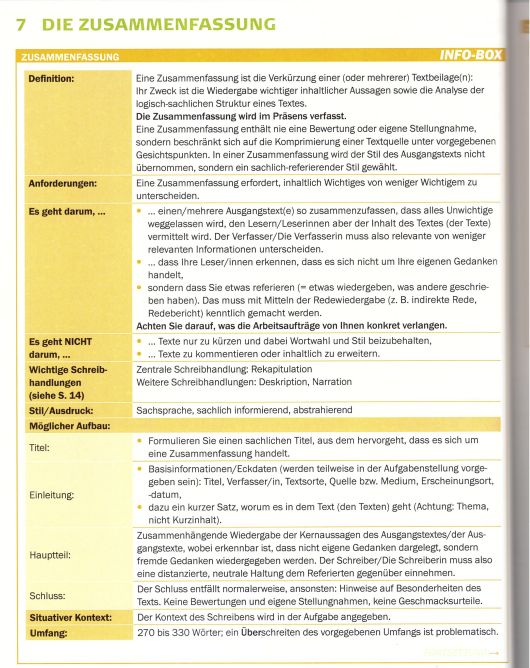
\includegraphics[scale=0.8]{./pics/Screenshot from 2023-02-06 12-32-33.png}
    \caption{Zusammenfassung: Definition + Aufbau}
    \label{fig:impl:Zusammenfassung1}
\end{figure}
\begin{figure}[h]
    \centering
    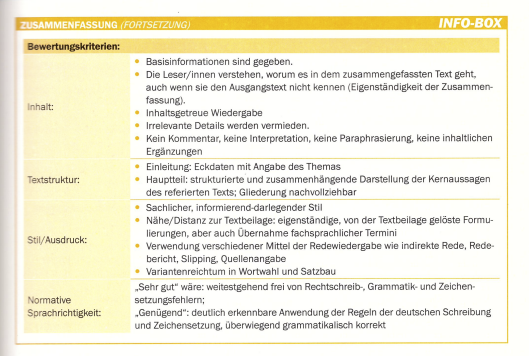
\includegraphics[scale=0.8]{./pics/Screenshot from 2023-02-06 12-33-05.png}
    \caption{Zusammenfassung: Verfassen}
    \label{fig:impl:Zusammenfassung2}
\end{figure}
\begin{figure}[h]
    \centering
    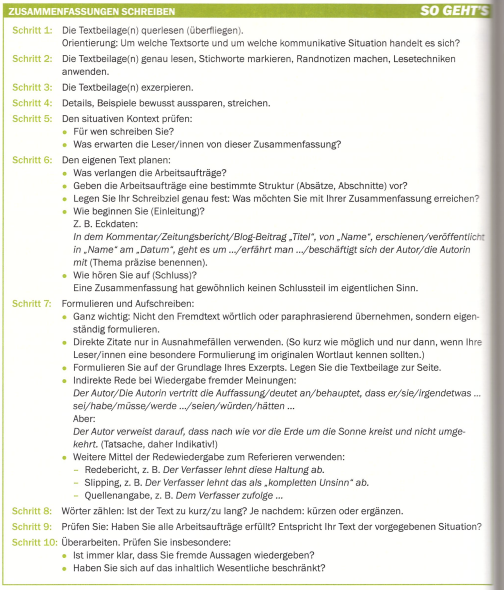
\includegraphics[scale=0.8]{./pics/Screenshot from 2023-02-06 12-33-47.png}
    \caption{Zusammenfassung: Fortsetzung}
    \label{fig:impl:Zusammenfassung3}
\end{figure}
  

\section{Mustertext}


\section{Eigener Text}

Lesen Sie den Zeitungsbericht „Die junge Generation ist benachteiligt“, der von Wolfgang Böhm verfasst wurde und in Die Presse am 13. November 2016 veröffentlicht wurde. Schreiben Sie nun eine Zusammenfassung und bearbeiten Sie folgende Arbeitsaufträge: Geben Sie die wichtigsten Inhalte hinsichtlich Jugendarbeitslosigkeit wieder. Beschreiben Sie die Vorzüge, die sich für die ältere Generation ergeben. Erschließen Sie die notwendigen Schritte, um einen sozialen Kollaps zu vermeiden.  

Schreiben Sie zwischen 270 und 330 Wörter. Markieren Sie Absätze mittels Leerzeilen 

\subsubsection{Die junge Generation ist benachteiligt!}
Der Artikel „Die junge Generation ist benachteiligt“ von Wolfgang Böhm (Die Presse), welcher am 13.11.2016 erschienen ist, handelt von den Auswirkungen der Finanzkriese 2007. Vor allem der große Unterschied zwischen den Jugendlichen und Menschen über 65 wurde stark herausgehoben.  

Konkret geht es darum, dass vor allem die Älteren es geschafft haben, eine gewisse Sicherheit zu wahren, während bei den Jungen die Unsicherheit und die Angst der Zukunft wuchs. In Zahlen ausgedrückt heißt es, dass während der Krise die Zahl der Arbeitslosen Jugendlichen bei 26.4 \% lag, sie danach bei 26.9\%. Im Vergleich, bei den über 65-Jährigen schrumpfte der Anteil von 23.3\% auf 17.4 Prozent. Auch in den Zahlen der schwerwiegenden Entbehrungen spiegelt sich die Situation wider. Während 9.5\% der Jugendlichen in Europa ihre Grundbedürfnisse nicht decken können, sind es bei den Älteren lediglich 5.5 Prozent. Auslöser dafür war während der Krise die Tatsache, dass sich die Gehälter und Pensionen älterer Arbeitnehmer kaum gekürzt wurden, jedoch das Einkommen der Jungen stark zurück ging.   

Laut der Studie ist die soziale der Jugend heute in keinem einzigen EU-Landbesser als im Jahr 2008. Österreich ist keine Ausnahme. Waren 2007 hier 16,7 Prozent der Kinder und Jugendlichen (bis zu 18 Jahren) von Armut oder sozialer Exklusion bedroht, so sind es heute 18,3 Prozent. Bei der Generation der über 65-Jährigen ging dieses Risiko von 21,2 auf 14 Prozent zurück. Auch besonders bemerkenswert ist das deutliche Nord-Süd-Gefälle. Jugendliche aus Nordeuropa haben noch eher Chancen auf einen Arbeitsplatz und ein geringeres Armutsrisiko als jene aus Südeuropa.  

Am Ende des Artikels wird zu Arbeitsmarkt und Bildungspolitik Reformen aufgerufen, da sich die Lage der Jugendlichen zu verschlechtern scheint. Kinder aus ärmeren Familien haben deutlich geringere Chancen, ein höheres Bildungsniveau zu erreichen als Kinder wohlhabender Eltern. Länder wie Finnland oder Estland seien hier vorbildlich. 
\section{Formulierungshilfen}

Einleitung:
enthält: Autor, Titel, Textsorte, Erscheinungsjahr/-datum, ggf. Erscheinungsort, kurze Benennung des Themas 
\begin{compactitem}
    \item Das/ Der /Die (Textsorte) „(Titel)“ von (Autor) aus dem Jahr .... beschreibt .../handelt von.../ thematisiert...  
    \item In dem (Zeitungsartikel) „(Titel)“ von (Autor) erschienen in (Erscheinungsort/ Herausgeber) am (Erscheinungsdatum) geht es um... 
\end{compactitem}
Hauptteil: 
\begin{compactitem}
    \item  Zu Beginn berichtet der Autor.../ spielt die Handlung... 
    \item  Anfangs wird festgestellt... / darauf hingewiesen, dass...
    \item  Eingangs .../ Zunächst.../ Bevor...
    \item Die Kurzgeschichte/ Der Roman/ Das Drama beginnt damit, dass... 
    \item Später geht der Autor darauf ein, dass... 
    \item  Im Folgenden... / Es folgt...
    \item Danach... / Später wird klar, dass...
    \item Im Verlauf der Geschichte/ des Berichtes/ des Kommentars etc. wird deutlich, dass...
    \item Plötzlich greift... in das Geschehen ein und.../ indem...
    \item  Die Situation beginnt sich zu verändern, als .../ nachdem... 
    \item Die Geschichte endet mit...
    \item Die Situation wird aufgelöst durch.../, indem.../ als..
    \item Schließlich .../ Am Ende.../ Zum Schluss... 
    \item Abschließend betont der Autor (nochmals), dass 
\end{compactitem}

Schluss:
\begin{compactitem}
    \item  Auf mich wirkt der Text... 
    \item  Zusammenfassend ist also pointiert festzuhalten, dass… 
    \item Letztlich bleibt anzumerken... 
    \item Als einzig logisches Fazit lässt sich also festhalten, dass...
    \item Abschließend ist daher anzunehmen, dass... 
    \item m Vergleich zu... ist es in diesem Text/ diesem Autor (nicht) gelungen... 
\end{compactitem}

\begin{spacing}{1}
	\chapter{Zusammenfassung}
\end{spacing}
\section{Fehlersammlung}

Übergänge und vor allem Rechtschreibung fällt mir schwer. Teilweise werde ich einfach zu unkonzentriert, und lese mir die Texte nicht mehr genau durch, und übersehe dadurch schnell kleine Fehler, die sich schnell zusammenläppern. Bei den Übergängen bin ich mir bei den Formulierungen oft nicht sicher, wie ich am besten eine flüssige Überleitung schreiben soll. Ich werde mir vor der Matura mehr von den Formulierungshilfen merken, um die Übergänge besser zu gestalten, und mir mehr Zeit zum Durchlesen nehmen. Inhaltlich gibt es kaum bis keine Probleme, aufpassen muss ich jedoch, dass der Inhalt zu den Aufgabenstellungen passt, und dass ich nicht einfach so drauf los schreibe. Dadurch kann der Text auch schnell mal zu lange werden, und mehr Fehler passieren. Da ich das aber niemals vorhersagen kann, werde ich einfach mehr üben müssen. Vor allem, weil ich oft in einen Flow reinkomme, wo mir das Schreiben guter Texte einfach fällt. Oft, aber nicht immer. Und dann sitzt ich manchmal da, und weiß nicht, was ich schreiben soll. 

Probleme bei dem Portfolio gab es hauptsächlich bei den neuen Texten, und vor allem auch zeitlich. Es war einfach sehr viel zu tun, wir haben alle viel zu spät angefangen. Selber schuld, werden Sie sich jetzt denken, aber es ging einfach nicht früher. Es war viel zu viel zu tun, und ich bin mir sicher, ich war nicht der Einzige, der kurz vor dem Zusammenbruch stand, weil er einfach viel zu überlastet war. Es wäre einfach nicht möglich gewesen, so viel früher anzufangen und somit mehr auf Fehler und Inhalt zu achten. Ich bin froh, dass ich so weit gekommen bin, eigentlich alles abgeschlossen habe. Ich bin nicht zufrieden, aber es ist da.  

\section{Schlusswort}
Viele der Textsorten waren keine große Herausforderung mehr, da wir sie die letzten Jahre oft und gut genug geübt haben. Einzig die Zusammenfassung und die Erörterung waren Probleme, da beide schon Jahre her sind. Verbessert habe ich mich vor allem bei den Formulierungen und meinem Ausdruck, da ich natürlich jetzt viel mehr Erfahrung als beim ersten Versuch habe.  

\section{Danksagung}
Am Ende dieser langen Reise möchte ich mich bei meinen liebsten bedanken. Bei Chen, meine Freundin, die mich immer motiviert hat, weiterzumachen. Sie war immer da, und vor allem in den schweren Zeiten hat es mir sehr geholfen, aufzustehen, und weiterzuschreiben. Außerdem möchte ich Lorenz danken, Lorenz aka die Lanze. Er war immer eine zuverlässige Quelle zu Informationen, und hat mir bei meiner Recherche sehr geholfen. Eine weitere wichtige Person auf dieser Reise war David Ursprung (auch als DJ XuX bekannt), der an dunklen Tagen immer den richtigen Musikmix bereit hatte. Philipp war ein Geist, der immer hinter einem stand, selbst wenn man ihn nicht sah. Sami hatte immer einen Überblick über alles, und half uns, alles zu koordinieren. Altenhofer David sorgte immer für die benötigte Ruhe im Klassenzimmer, während uns Mathias mit seinen Witzen immer unterhalten hatte. Dave war wie eine Mentale stütze, und wusste immer, jeden zu motivieren. Immer an seiner Seite war Ema, die nicht nur die Mutter der Klasse war, sondern jeden wieder zurück ins Leben gerufen hatte. Fabian Maar war der Analytische, der Ruhige. Er unterstütze jeden, wo er nur konnte, und schrieb still und heimlich an seinem Portfolio. Ana sorgte für die willkommene Abwechslung, mit lustigen Sprüchen und frechen Kommentaren. Annika konnte die Klasse mit dem besten Essen versorgen, während wir alle Stundenlang über unseren Laptops hingen.  Fabian Ettinger war der Professionelle, der immer genug Energie (drinks) für die ganze Klasse hatte. Im Speedrun Style hat er das Portfolio innerhalb weniger Tagen aus seinem Kopf gezaubert. Dominik war der Träumer, er träumte von einer Welt, wo nur die ganze Klasse zusammen ein Portfolio schreiben muss. Doch er stand immer hinter einem, und hat jeden unterstütz.  

 
\newpage
\section{Quellen}

Erörterung Aufgabenstellungen: 

\href{https://prod.aufgabenpool.at/srdp\_vgs/aufgaben/60/KL18\_PT1\_DEU\_3.1\_AU.pdf}{https://prod.aufgabenpool.at/srdp\_vgs/aufgaben/60/KL18\_PT1\_DEU\_3.1\_AU.pdf}  

Kommentar Erklärung:  \href{https://www.deutsche-grammatik.net/textsorten-srdp/kommentar/ }{www.deutsche-grammatik.net/textsorten-srdp/kommentar/ }

Kommentar Aufgabenstellung

\href{https://prod.aufgabenpool.at/srdp\_vgs/aufgaben/267/KL22\_PT1\_DEU\_2.2\_AU.pdf}{https://prod.aufgabenpool.at/srdp\_vgs/aufgaben/267/KL22\_PT1\_DEU\_2.2\_AU.pdf}

Beispieltext der Zusammenfassung: \href{https://www.scribbr.de/studium/zusammenfassung-schreiben/}{https://www.scribbr.de/studium/zusammenfassung-schreiben/}

Aufgabenstellung zur Zusammenfassung:

\href{https://www.deutsche-grammatik.net/app/download/19417237025/Zusammenfassung\_Die+junge+Generation+ist+benachteiligt.pdf?t=1666362281 }{https://www.deutsche-grammatik.net/app/download/}

Kommentar: \href{ https://www.deutsche-grammatik.net/textsorten-srdp/kommentar/}{ https://www.deutsche-grammatik.net/textsorten-srdp/kommentar/}

Aufgabenpool: \href{https://prod.aufgabenpool.at/srdp/startseite/}{https://prod.aufgabenpool.at/srdp/startseite/}

Informationen zu den einzelnen Textsorten: 

\href{https://www.matura.gv.at/index.php?eID=dumpFile\&t=f\&f=4525\&token=950c7f2b86f0ebc3459c5f0aa0e04013ab99c572}{https://www.matura.gv.at/}

Weitere wichtige Links:

\href{https://www.schreiben.net/}{https://www.schreiben.net/}

\href{https://www.studysmarter.de/schule/deutsch/textproduktion/leserbrief/ }{https://www.studysmarter.de/schule/deutsch/textproduktion/leserbrief/ }

\href{https://wortwuchs.net/kommentar/ }{https://wortwuchs.net/kommentar/ }

\href{https://besser-deutsch.com/mit-diesen-tipps-gelingt-deine-meinungsrede-bestimmt/#:~:text=Im%20Gegensatz%20zu%20anderen%20Textsorten,keine%20allzu%20komplexen%20Satzstrukturen%20verwenden. }{https://besser-deutsch.com/}

\href{https://www.deutsche-grammatik.net/ }{https://www.deutsche-grammatik.net/ }

\href{https://www.imst.ac.at/imst-wiki/images/f/f2/Rohfassung_hilfe_textkommentare.pdf }{https://www.imst.ac.at/}


\input{./sections/appendix}
\end{document}

